\documentclass[oneside]{scrbook} %KOMA-Script book
\usepackage[italian]{babel}
%Per i commenti
\usepackage{comment}
%Per l'interlinea
\usepackage{setspace}
%Codifica caratteri
\usepackage[utf8]{inputenc}
\usepackage{xspace}
\usepackage{eurosym}
%Fonts Scientifici
\usepackage{amsfonts}
\usepackage{amsmath}
\usepackage{amssymb}
\usepackage{textcomp}
%Pacchetto grafici
\usepackage{tikz}
\usepackage{pgfplots}
\pgfplotsset{/pgf/number format/use comma,compat=newest}
\usepackage{picture}
\usepackage{graphicx}
%Impostazioni tabelle avanzate e colorate
\usepackage{multicol}
\usepackage{multirow}
\usepackage{soul}
\usepackage{ulem}
\usepackage{booktabs}
%\usepackage{subfig}
\usepackage{subfigure}
\usepackage{array}
\usepackage{color}
\usepackage{colortbl}
%Pacchetto per gli pseudocodici
\usepackage{algpseudocode}
%\usepackage{listings}
\usepackage{listings,xcolor,courier,bookmark}
\usepackage{listingsutf8}
%Impostazioni tabelle avanzate
\usepackage{multicol}
\usepackage{multirow}
\usepackage{rotating}
\definecolor{darkblue}{named}{blue}
\definecolor{darkred}{named}{red}
\definecolor{grau}{named}{gray}
%Per i margini
\usepackage{chngpage}
\sloppy

\graphicspath{{Immagini/}}

\let\Righttorque\relax

\lstset{
	captionpos=b,
	commentstyle=\color[rgb]{0.133,0.545,0.133},
	keywordstyle=\color{darkblue},
	stringstyle=\color{purple},
	extendedchars=true,
	basicstyle=\small\ttfamily,
	showstringspaces=false,
	tabsize=2,
	numbers=left,
	numberstyle=\tiny,
	breakautoindent  = true,
	breakindent      = 2em,
	breaklines       = true,
	postbreak        = ,
	prebreak         = \raisebox{-.8ex}[0ex][0ex]{\Righttorque},
	showspaces=false,
	showtabs=false,
	showstringspaces=false,
	language=C++,
	frame=single,
	morecomment=[s]{°°},
	inputpath=Sorgenti/
}

\renewcommand*{\lstlistingname}{Codice}
\renewcommand*{\lstlistlistingname}{Elenco dei codici}

\usepackage{fancyhdr}
\pagestyle{fancy}
\renewcommand{\chaptermark}[1]{\markboth{\MakeUppercase{\thechapter.\ #1}}{}}
\fancypagestyle{plain} %stile delle pagine anche a quella iniziale del capitolo

\fancyhead{}
\fancyfoot{}

\fancyhead[R]{\bfseries \nouppercase{\leftmark}}
\fancyhead[L]{
	\includegraphics*[scale=0.8]{logo_dieti2.png}
}
\fancyfoot[R]{\thepage}
\fancyfoot[L]{Tesina di Impianti di Elaborazione}
\renewcommand{\headrulewidth}{0.4pt}
\renewcommand{\footrulewidth}{0.4pt}

\date{}
\cfoot{}
\usepackage{eso-pic,graphicx}

%Per sottosezioni
\setcounter{secnumdepth}{4}
\setcounter{tocdepth}{4}

\begin{document}

	% Per evitare che i collegamenti nell'indice abbiano i riquadri rossi
	\hypersetup {linkbordercolor=white}

	\AddToShipoutPicture{\AtPageCenter{\makebox(0,0){
\includegraphics{logo.png}}}}
	\frontmatter
	\pagenumbering{Roman}

	\begin{titlepage}
		\centering
		%{\Huge \textsc{Università degli Studi di Napoli ``Federico II''}}

		%\vspace*{\stretch{2.5}}

		%
\includegraphics[width=1\linewidth]{logo_federico_II.png}

		
\includegraphics[width=1\linewidth]{logo_dieti2.png}

		\vspace*{2cm}

		{\Huge \textsl{Tesina di\\IMPIANTI DI ELABORAZIONE}\par}

		\vspace*{2cm}

		{\huge \text{Prof. Domenico Cotroneo}}

		\vspace*{5cm}

		{\LARGE \textit{Andrea Scognamiglio - Matr. M63/598\\Cristian Tommasino - Matr. M63/615}}

		\vspace*{2.5cm}

		{\Large \textsc{A.A. 2017/2018}}
	\end{titlepage}

	\setcounter{page}{1}

	\newpage
	\tableofcontents

	\newpage
	\mainmatter
	
	% !TEX root = ./main.tex
% !TEX encoding = UTF-8 Unicode
% !TEX program = pdflatex
% !TeX spellcheck = it_IT

\graphicspath{{Immagini/},{Immagini/prodotto_matrici/}}

\chapter{Prodotto Matrici}

\section{Traccia}
Confrontare in Java e in C++ l'esecuzione del prodotto di matrici quadrate
di dimensione: 10000, 100000, 1000000.\\
Tale benchmark è utilizzato per valutare le prestazione dei
due linguaggi di programmazione.\\

\section{System Under Test}
La macchina target utilizzata per l'esecuzione degli algoritmi è:
\begin{itemize}
  \item \textbf{Processore}: Intel(R) Core(TM) i7-7700HQ @ 2.80GHz
  \item \textbf{Memoria Ram}: 16GB DDR4-2400MHz
  \item \textbf{Tipo sistema}: Windows 10 64bit, processore basato su x64
  \item \textbf{Storage}: SSD Kingston M.2.SATA 480GB
\end{itemize}

\section{Soluzione}
Il classico algoritmo di prodotto matriciale(\textbf{IKJ Algorithm}), ha una complessità computazionale
$O(n^3)$, dunque, per le dimensioni assegnate, richiederebbe un tempo di esecuzione
elevato.\\
Per questo motivo si è scelto di ridurre notevolmente le dimensioni delle matrici
ed utilizzare l'algoritmo di \textbf{Strassen}, avente complessità computazionale $O(n^{2,81})$.\\

\subsection{Strassen Algorithm}
L'algoritmo di Strassen calcola il prodotto di matrici quadrate assumendo che siano
del tipo $2^n \times 2^n$. \\ In particolare: $C=A \cdot B$ con $A,B,C \in R^{2^n \times 2^n}$.\\
Dividendo le matrici A,B e C in blocchi si ottiene:
\\
\[
A =
\begin{bmatrix}
  A_{1,1} & A_{1,2} \\
  A_{2,1} & A_{2,2}
\end{bmatrix}
B =
\begin{bmatrix}
  B_{1,1} & B_{1,2} \\
  B_{2,1} & B_{2,2}
\end{bmatrix}
C =
\begin{bmatrix}
  C_{1,1} & C_{1,2} \\
  C_{2,1} & C_{2,2}
\end{bmatrix}
\]\\
con $A, B, C \in R^{2^{n-1} \times 2^{n-1}}$.\\
\\
La matrice risultato si ottiene come:\\
$$C_{1,1} = A_{1,1}B_{1,1}+A_{1,2}B_{2,1}$$
$$C_{1,2} = A_{1,1}B_{1,2}+A_{1,2}B_{2,2}$$
$$C_{2,1} = A_{2,1}B_{1,1}+A_{2,2}B_{2,1}$$
$$C_{2,2} = A_{2,1}B_{1,2}+A_{2,2}B_{2,2}$$
\\
Utilizzando tale tecnica, il numero di prodotti matriciali da svolgere è 8.\\
Al fine di ridurre il numero di moltiplicazioni necessarie a generare le matrici
$C_{x,y}$, è possibile definire le seguenti
matrici:\\
$$M_1 = (A_{1,1}+A_{2,2})(B_{1,1}+B_{2,2})$$
$$M_2 = (A_{2,1}+A_{2,12})B_{1,1}$$
$$M_3 = A_{1,1}(B_{1,2}-B_{2,2})$$
$$M_4 = A_{2,2}(B_{2,1}-B_{1,1})$$
$$M_5 = (A_{1,1}+A_{1,2})B_{2,2}$$
$$M_6 = (A_{2,1}-A_{1,1})(B_{1,1}+B_{1,2})$$
$$M_7 = (A_{1,2}-A_{2,2})(B_{2,1}+B_{2,2})$$
Quindi la matrice risultato si ottime come:
$$C_{1,1} = M_1 + M_4 - M_5 + M_7$$
$$C_{1,2} = M_3 + M_5$$
$$C_{2,1} = M_2 + M_4$$
$$C_{2,2} = M_1 - M_2 + M_3 + M_6$$

\clearpage
\section{Analisi}

Gli algoritmi sono stati testati su matrici quadrate di dimensione 1024, 2048 e 4096.\\
Come analisi preliminare sono state effettuate 5 osservazioni indipendenti, al variare di N.\\
Per rendere le esecuzioni indipendenti, gli algoritmi sono stati eseguiti tramite uno
script batch.\\
L'algoritmo in Java è stato testato anche disattivando il \textbf{JIT}(Just In Time)
compiler, il quale ottimizza l'esecuzione dell'algoritmo, e in C++ abilitando anche
l'ottimizzazione \textbf{O2} (per codice più veloce e snello).\\

\subsection{Numero di esperimenti}

Per determinare la dimensioni dei campioni si è fatto utilizzo della seguente formula:
$$N= {\biggl({{\frac{100*z*s}{r*\overline{x}}}\biggr)}^2}$$
Dove:
\begin{itemize}
  \item \textbf{\textit{z}}: $(1-{\alpha / 2})$-quantile della distribuzione normale
  per ottenere un intervallo di confidenza $100\cdot(1-\alpha)$;
  \item \textbf{\textit{s}}: deviazione standard del campione;
  \item \textbf{\textit{r}}: accuratezza percentuale;
  \item \textbf{{$\overline{\textit{x}}$}}: media del campione.
\end{itemize}

Nel caso in analisi, l'intervallo di confidenza desiderato è del 95\%, quindi
$\alpha = 0.05$ ed $ r = 5 $.

Nelle seguenti figure sono riportati i tempi raccolti e le relative statistiche
utilizzate per la valutazione del parametro \textbf{N}.
\begin{figure}[!htbp]
  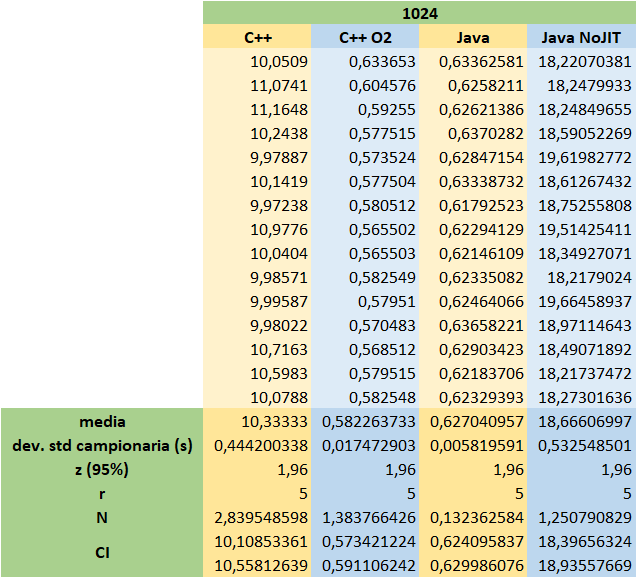
\includegraphics[width=1\linewidth,keepaspectratio]{tempi_1024}
  \caption{Esperimenti matrici 1024x1024}
  \label{prodottomatrici_tempi_1024}
\end{figure}

\begin{figure}[!htbp]
  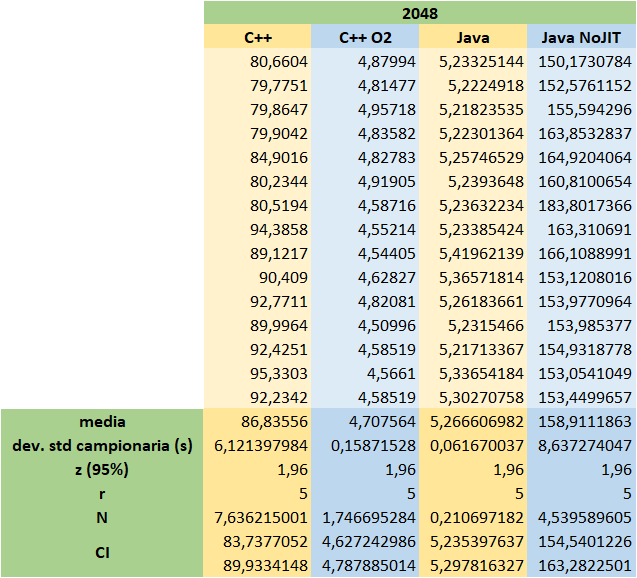
\includegraphics[width=1\linewidth,keepaspectratio]{tempi_2048}
  \caption{Esperimenti matrici 2048x2048}
  \label{prodottomatrici_tempi_2048}
\end{figure}

\begin{figure}[!htbp]
  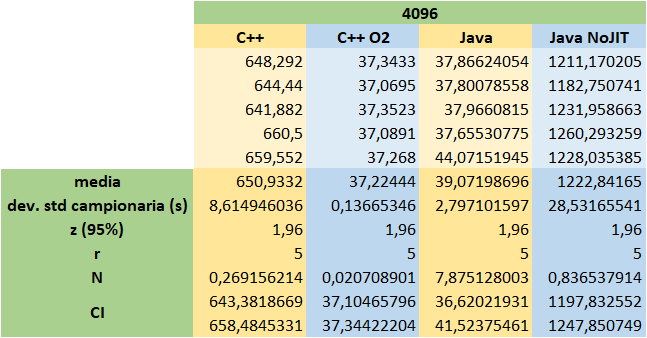
\includegraphics[width=1\linewidth,keepaspectratio]{tempi_4096}
  \caption{Esperimenti matrici 4096x4096}
  \label{prodottomatrici_tempi_4096}
\end{figure}

\clearpage

A valle dei 5 esperimenti svolti al variare della dimensione delle matrici,
considerando il caso peggiore, il numero di esperimenti necessario,
risulta essere 8.\\

\subsection{Esperimenti}

Nelle figure seguenti sono riportati i tempi di esecuzione degli 8 esperimenti
sull'algoritmo di Strassen, svolto nei differenti linguaggi.\\

\begin{figure}[!htbp]
  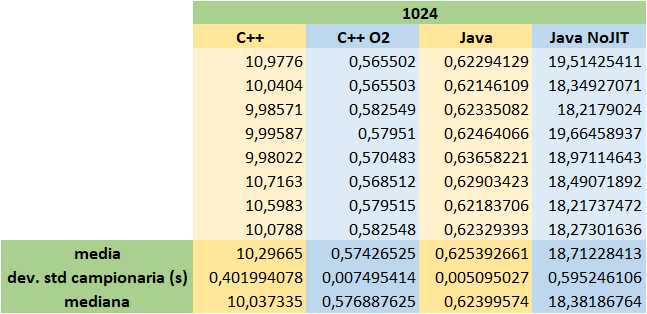
\includegraphics[width=1\linewidth,keepaspectratio]{tempi_8_1024}
  \caption{Esperimenti matrici 1024x1024}
  \label{prodottomatrici_tempi_8_1024}
\end{figure}

\begin{figure}[!htbp]
  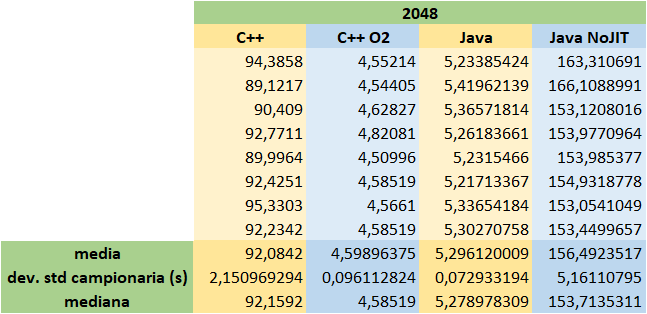
\includegraphics[width=1\linewidth,keepaspectratio]{tempi_8_2048}
  \caption{Esperimenti matrici 2048x2048}
  \label{prodottomatrici_tempi_8_2048}
\end{figure}

\begin{figure}[!htbp]
  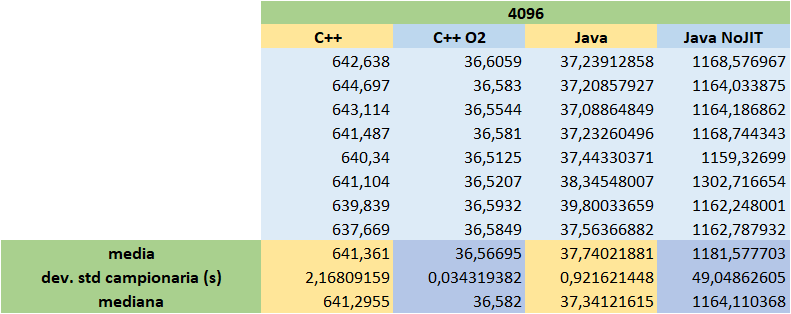
\includegraphics[width=1\linewidth,keepaspectratio]{tempi_8_4096}
  \caption{Esperimenti matrici 4096x4096}
  \label{prodottomatrici_tempi_8_4096}
\end{figure}

\clearpage

In seguito sono riportati i grafici del confronto dei tempi di Java e C++, sia
nelle loro versioni ottimizzate dal compilatore sia in quelle non ottimizzate.\\

\begin{figure}[!htbp]
  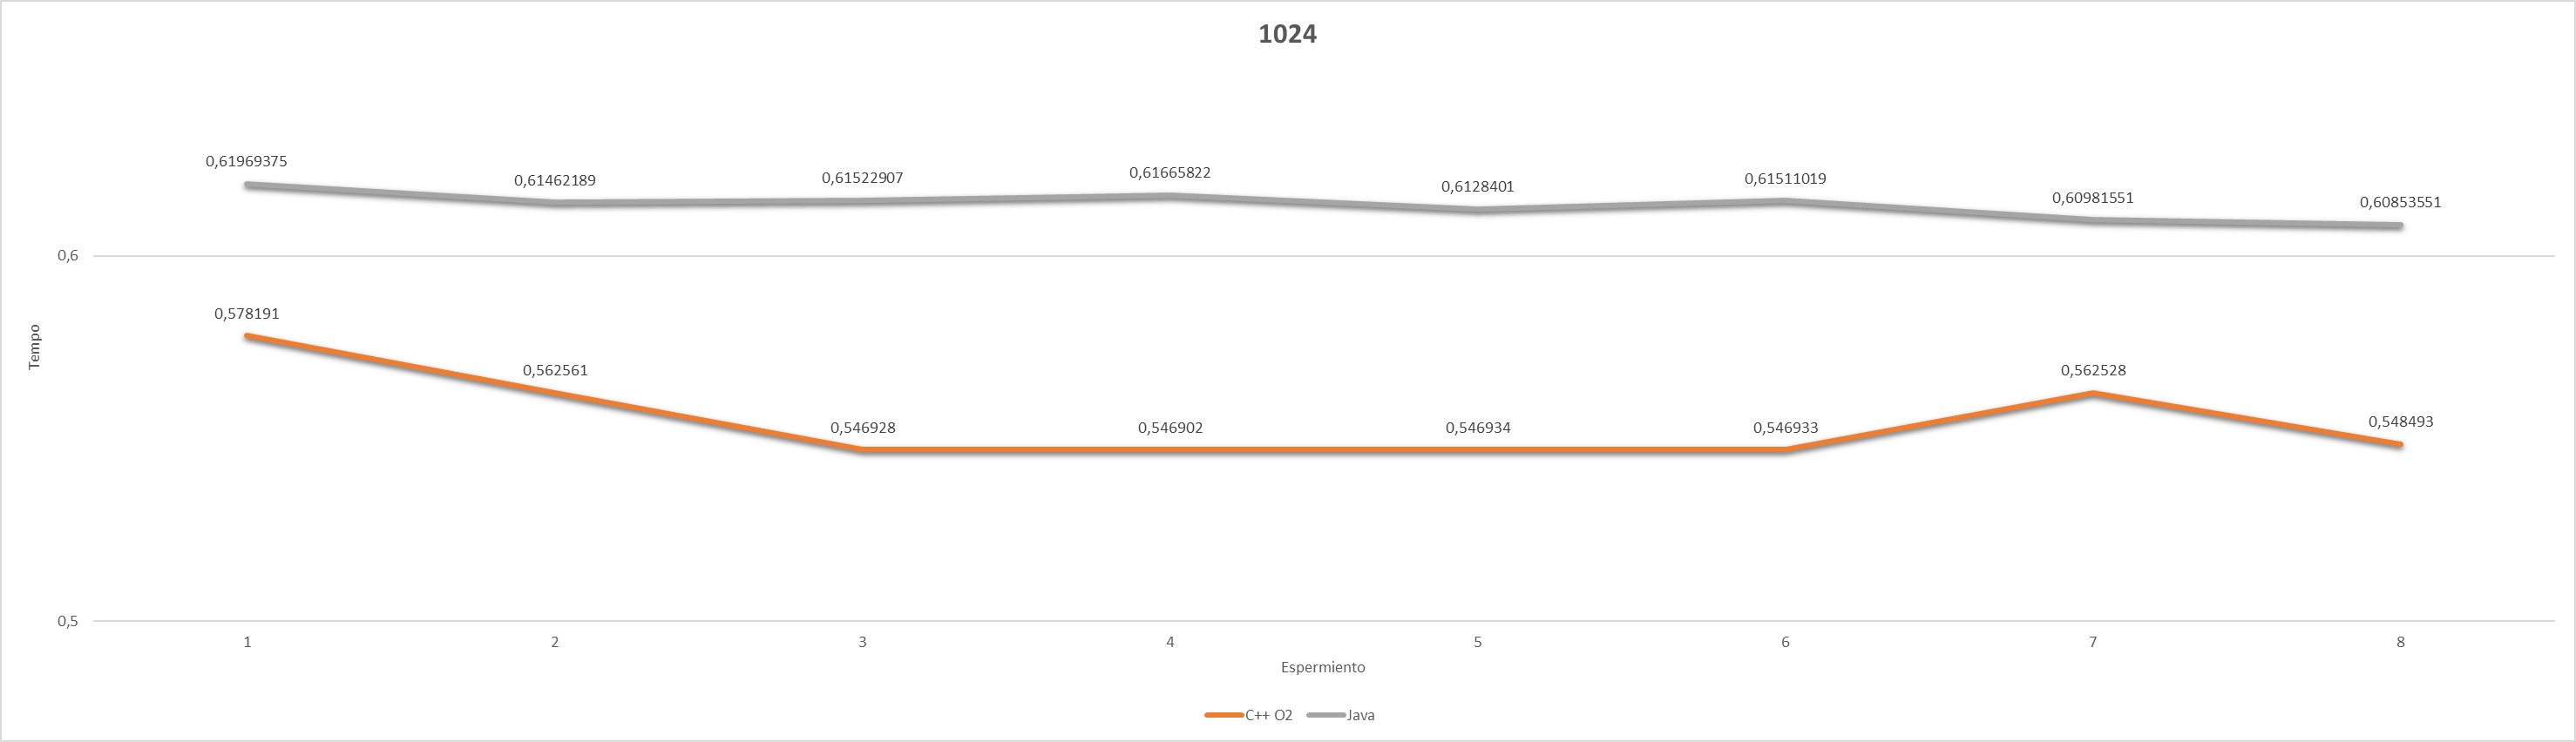
\includegraphics[width=1\linewidth,keepaspectratio]{grafico_tempi_1024_2}
  \caption{Confronto tempi \textbf{Java} vs \textbf{C++ O2} 1024x1024}
  \label{prodottomatrici_grafico_tempi_1024_2}
\end{figure}

\begin{figure}[!htbp]
  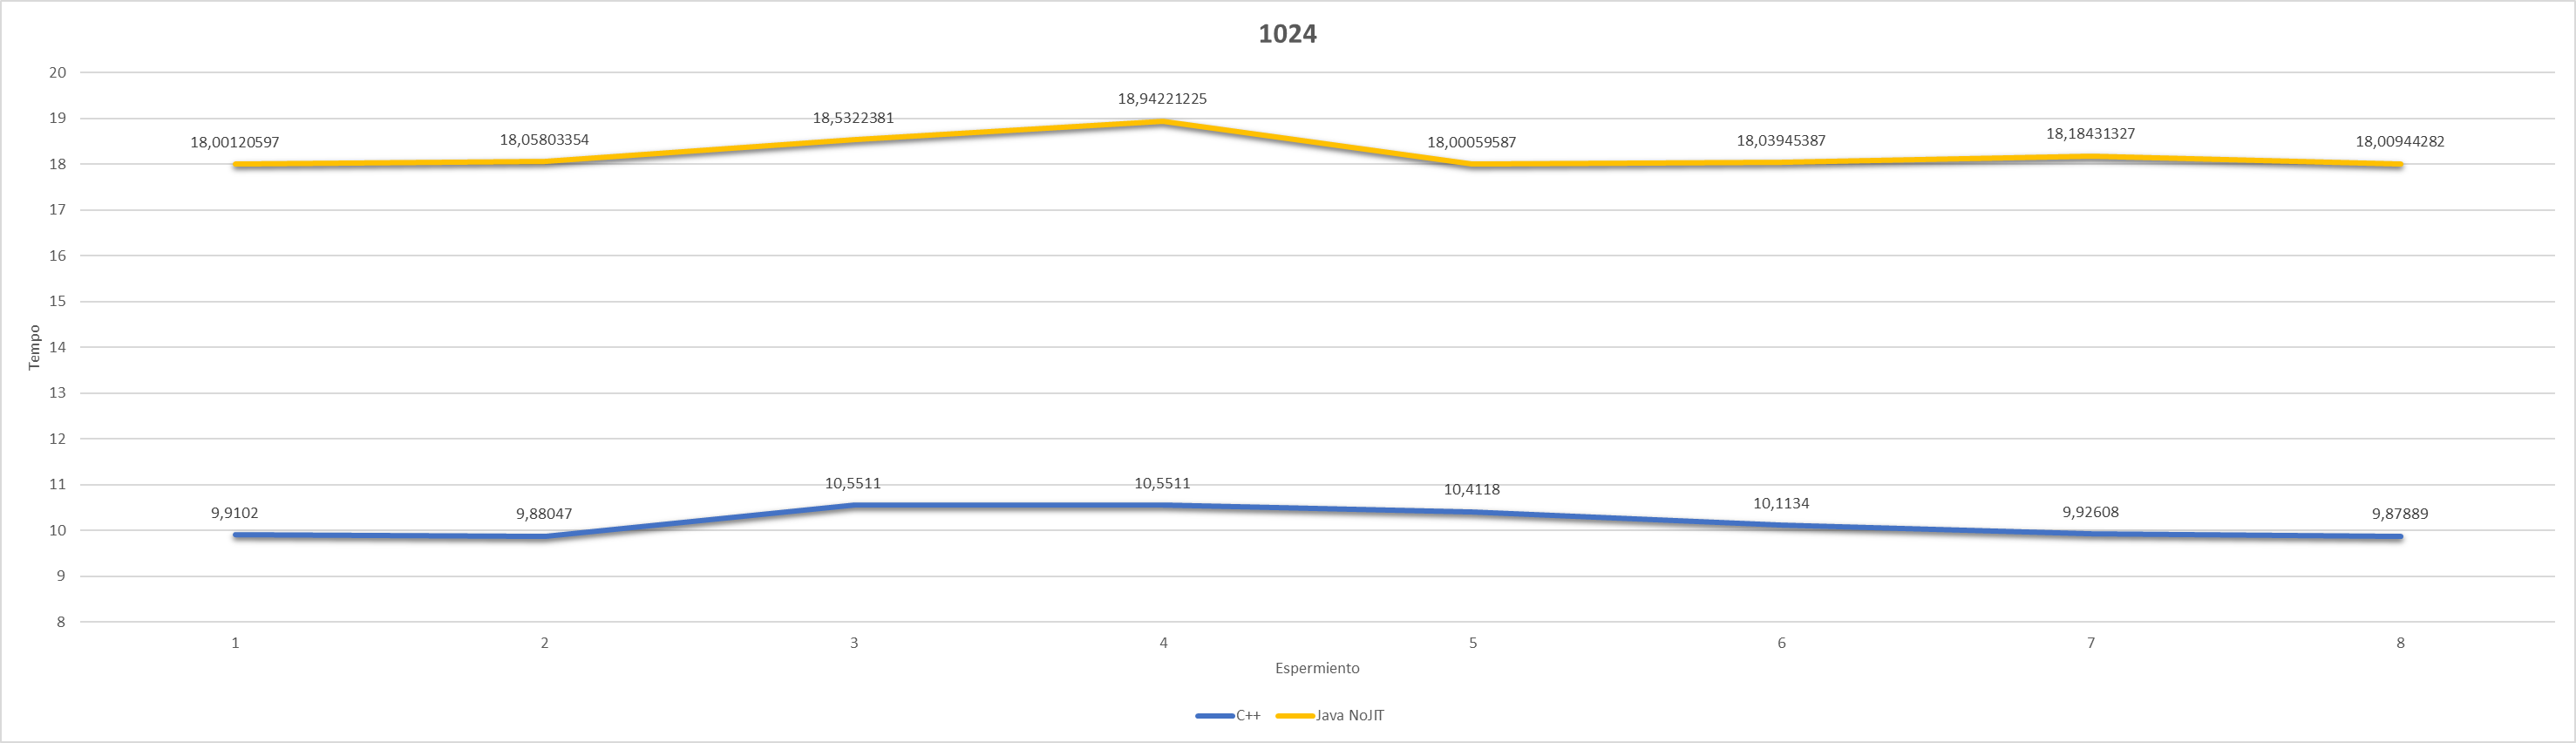
\includegraphics[width=1\linewidth,keepaspectratio]{grafico_tempi_1024_1}
  \caption{Confronto tempi \textbf{Java NoJIT} vs \textbf{C++} 1024x1024}
  \label{prodottomatrici_grafico_tempi_1024_1}
\end{figure}

\clearpage

\begin{figure}[!htbp]
  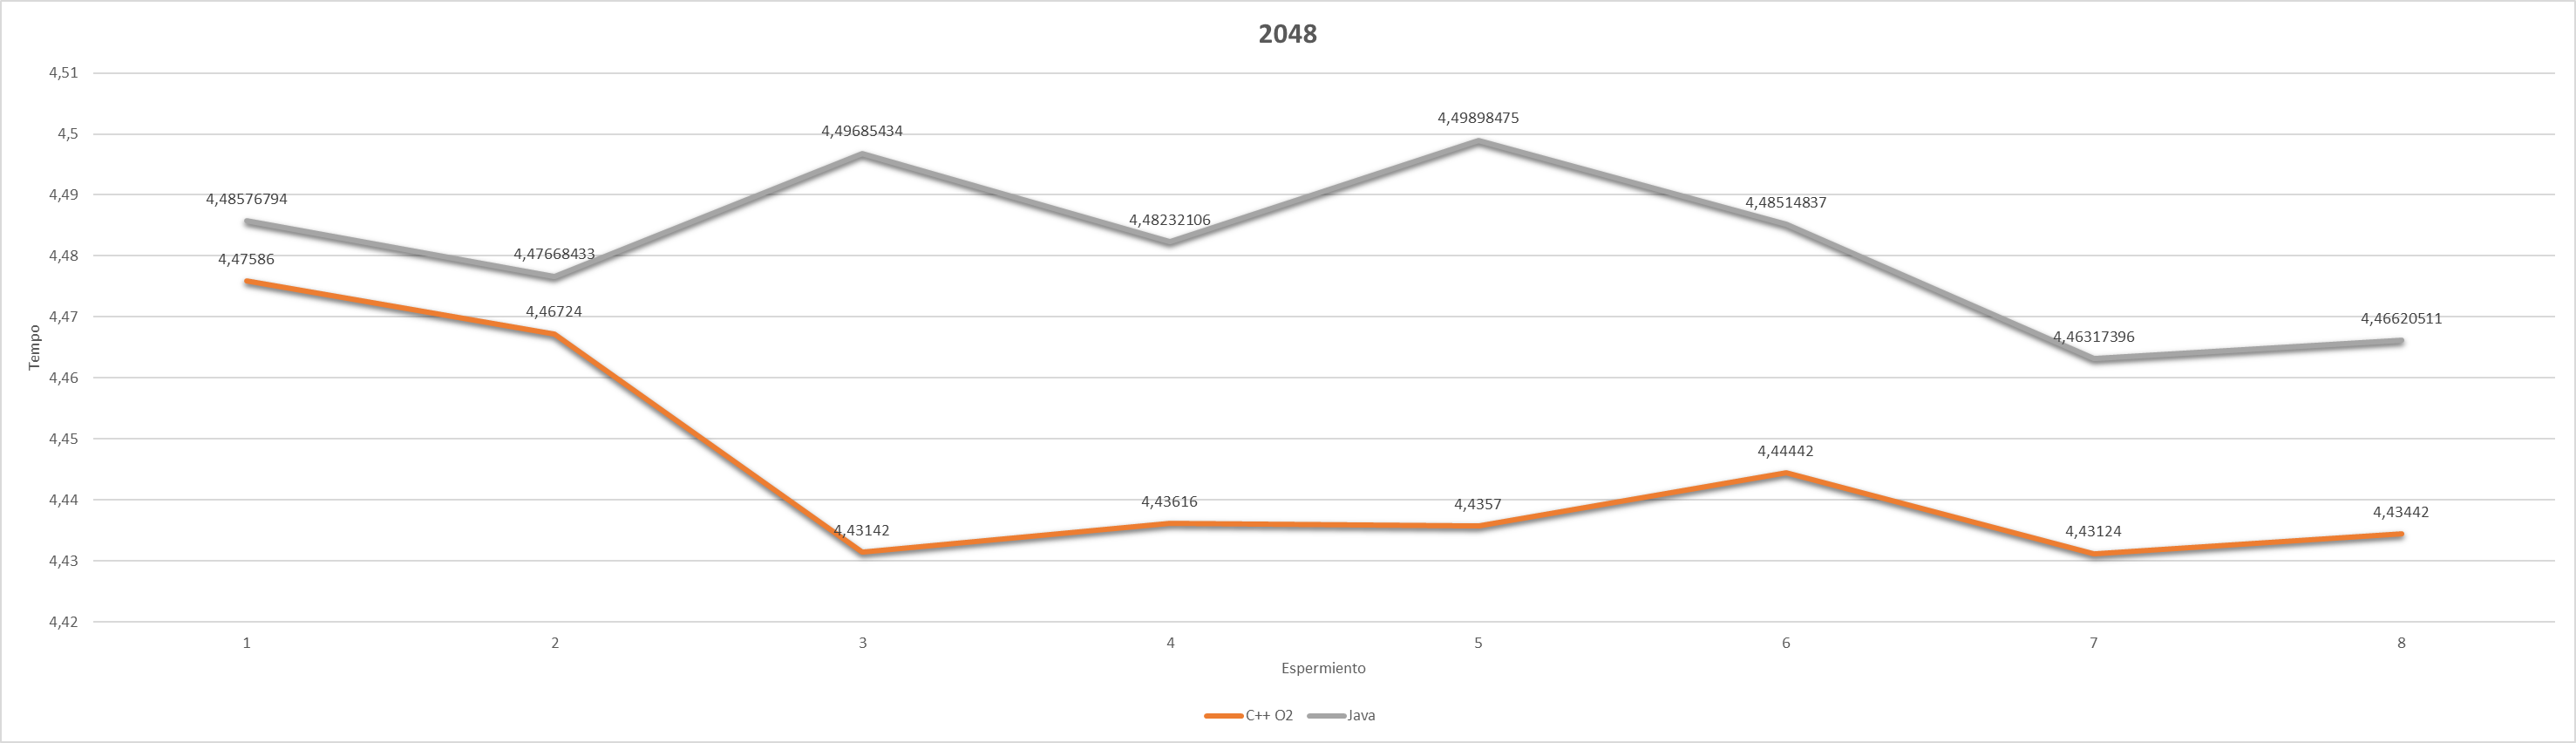
\includegraphics[width=1\linewidth,keepaspectratio]{grafico_tempi_2048_2}
  \caption{Confronto tempi \textbf{Java} vs \textbf{C++ O2} 2048x2048}
  \label{prodottomatrici_grafico_tempi_2048_2}
\end{figure}

\begin{figure}[!htbp]
  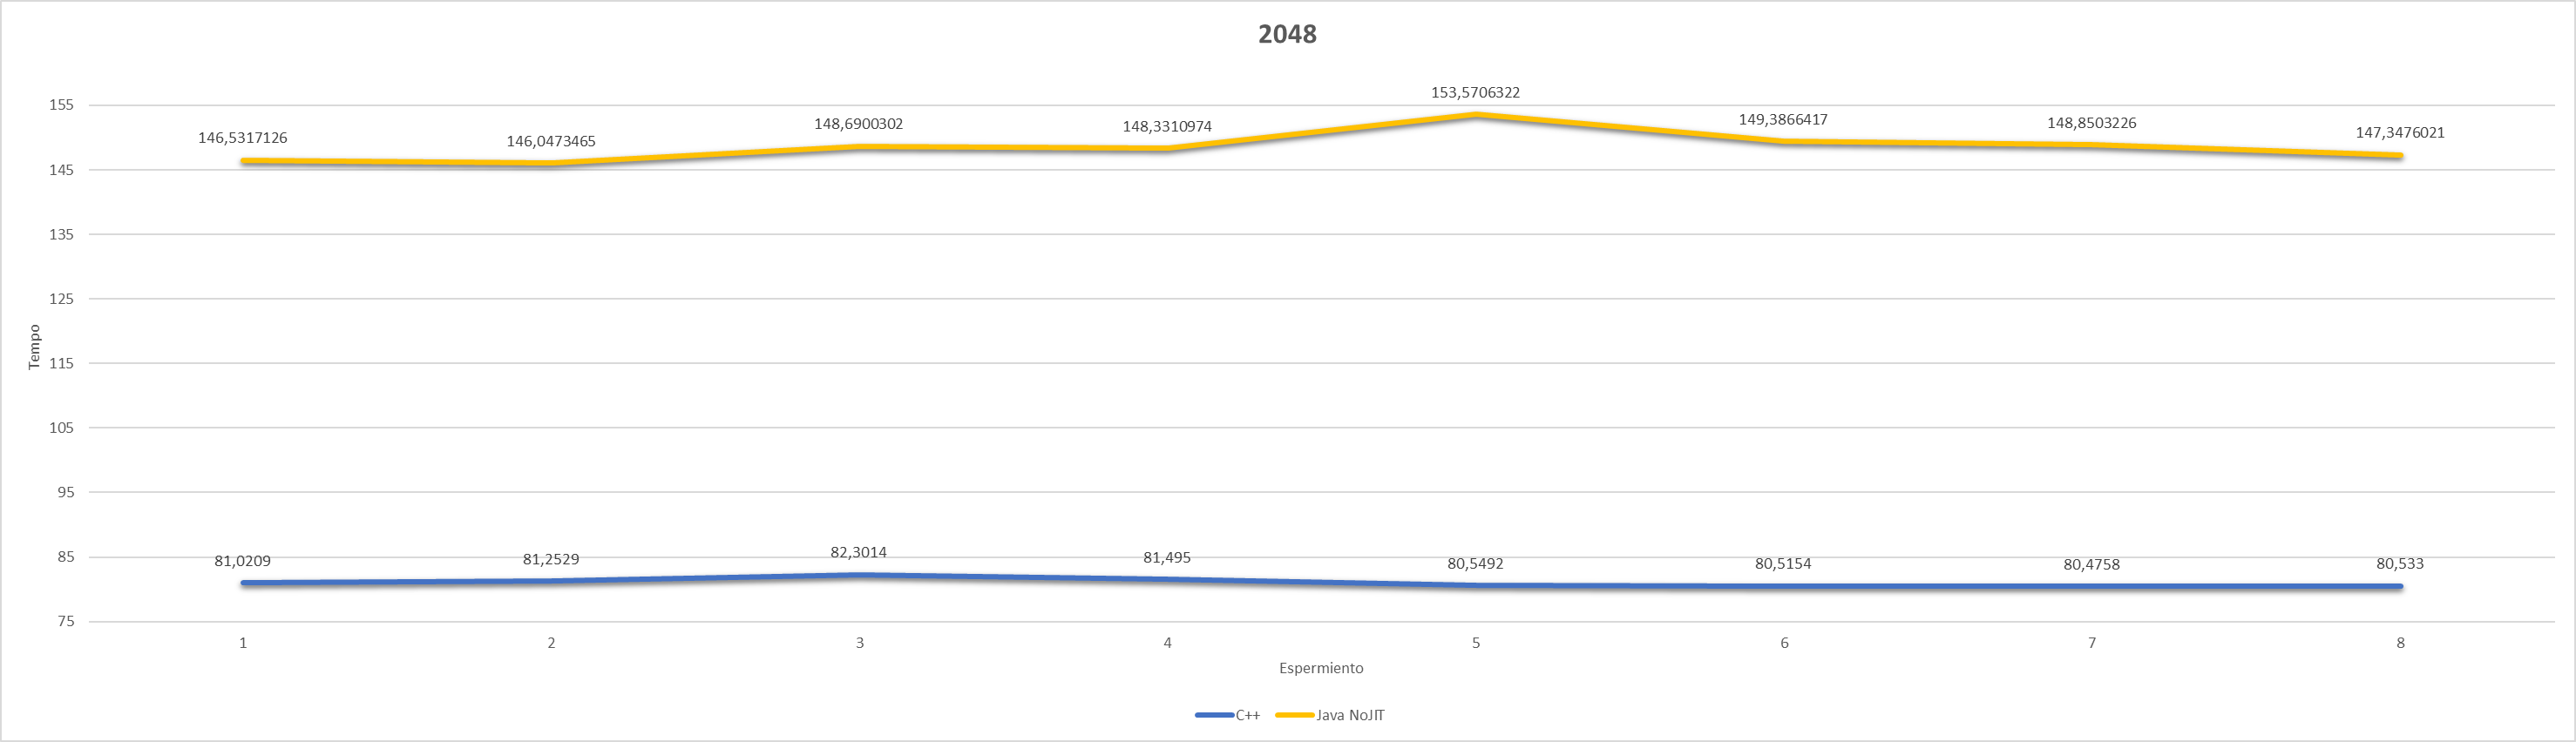
\includegraphics[width=1\linewidth,keepaspectratio]{grafico_tempi_2048_1}
  \caption{Confronto tempi \textbf{Java NoJIT} vs \textbf{C++} 2048x2048}
  \label{prodottomatrici_grafico_tempi_2048_1}
\end{figure}

\clearpage

\begin{figure}[!htbp]
  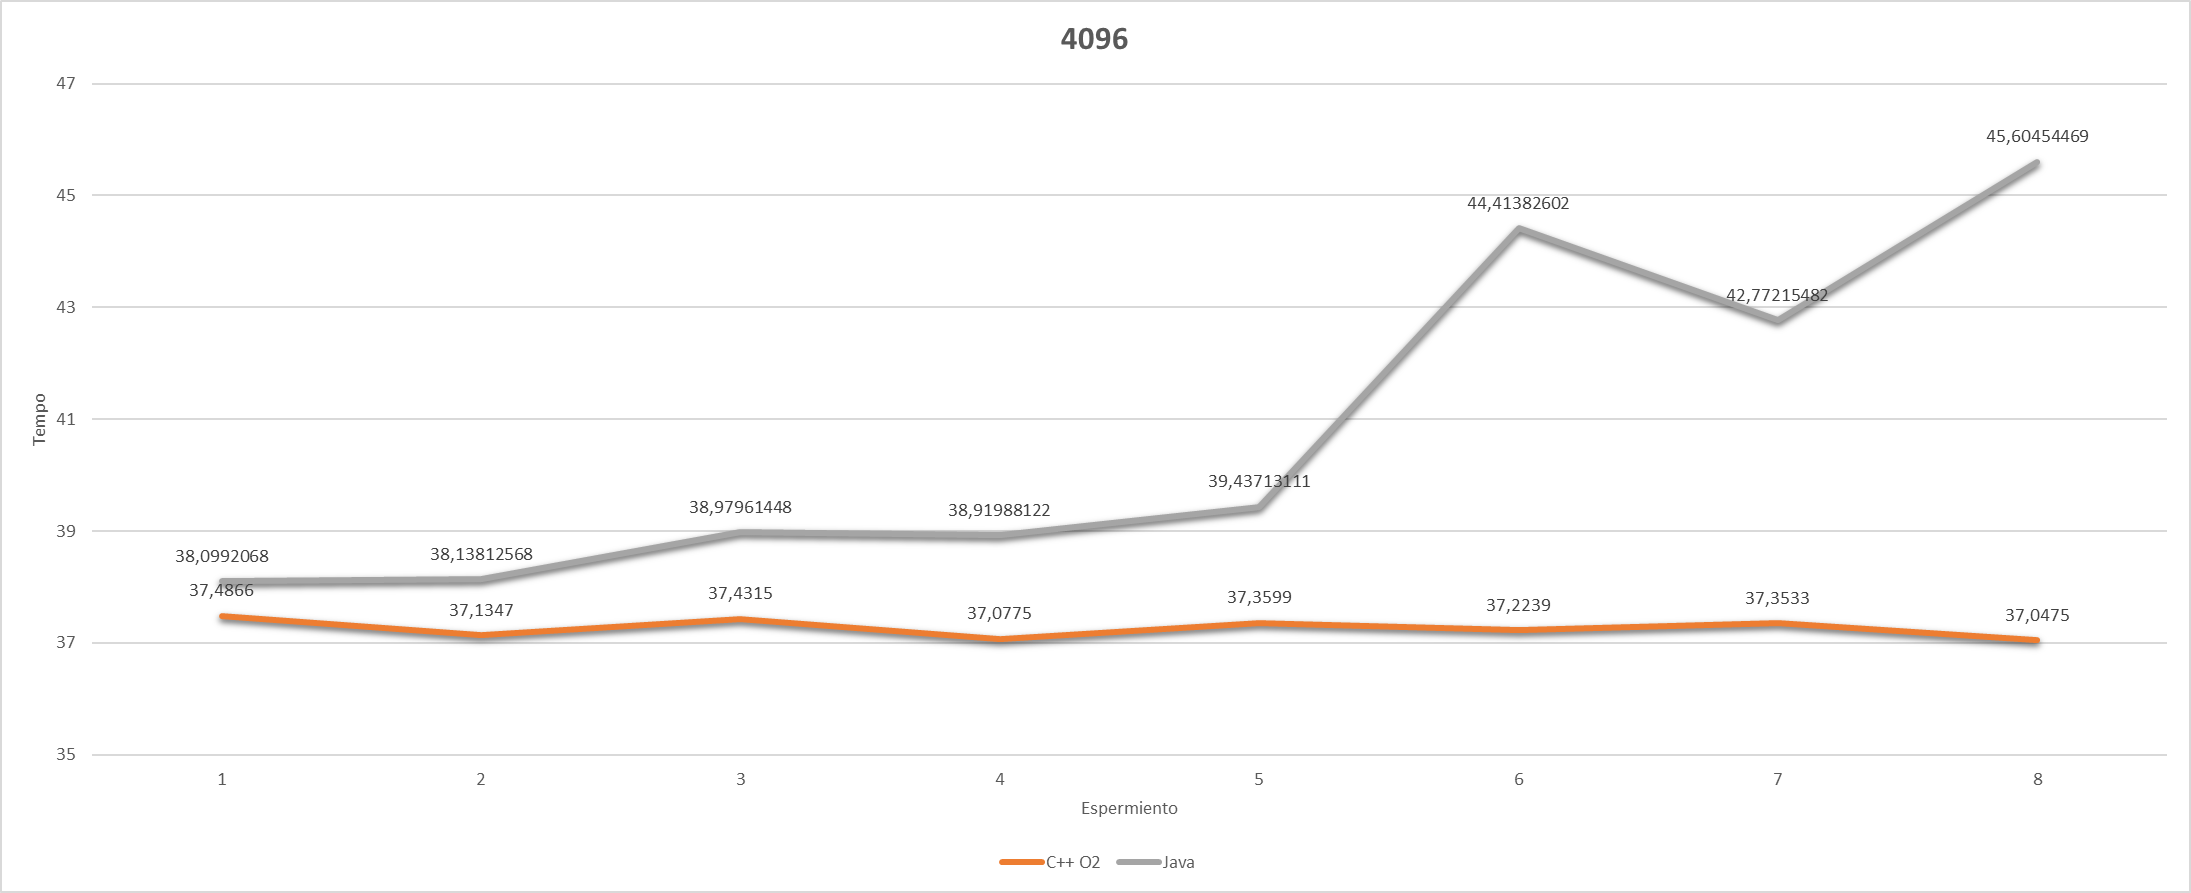
\includegraphics[width=1\linewidth,keepaspectratio]{grafico_tempi_4096_2}
  \caption{Confronto tempi \textbf{Java} vs \textbf{C++ O2} 4096x4096}
  \label{prodottomatrici_grafico_tempi_4096_2}
\end{figure}

\begin{figure}[!htbp]
  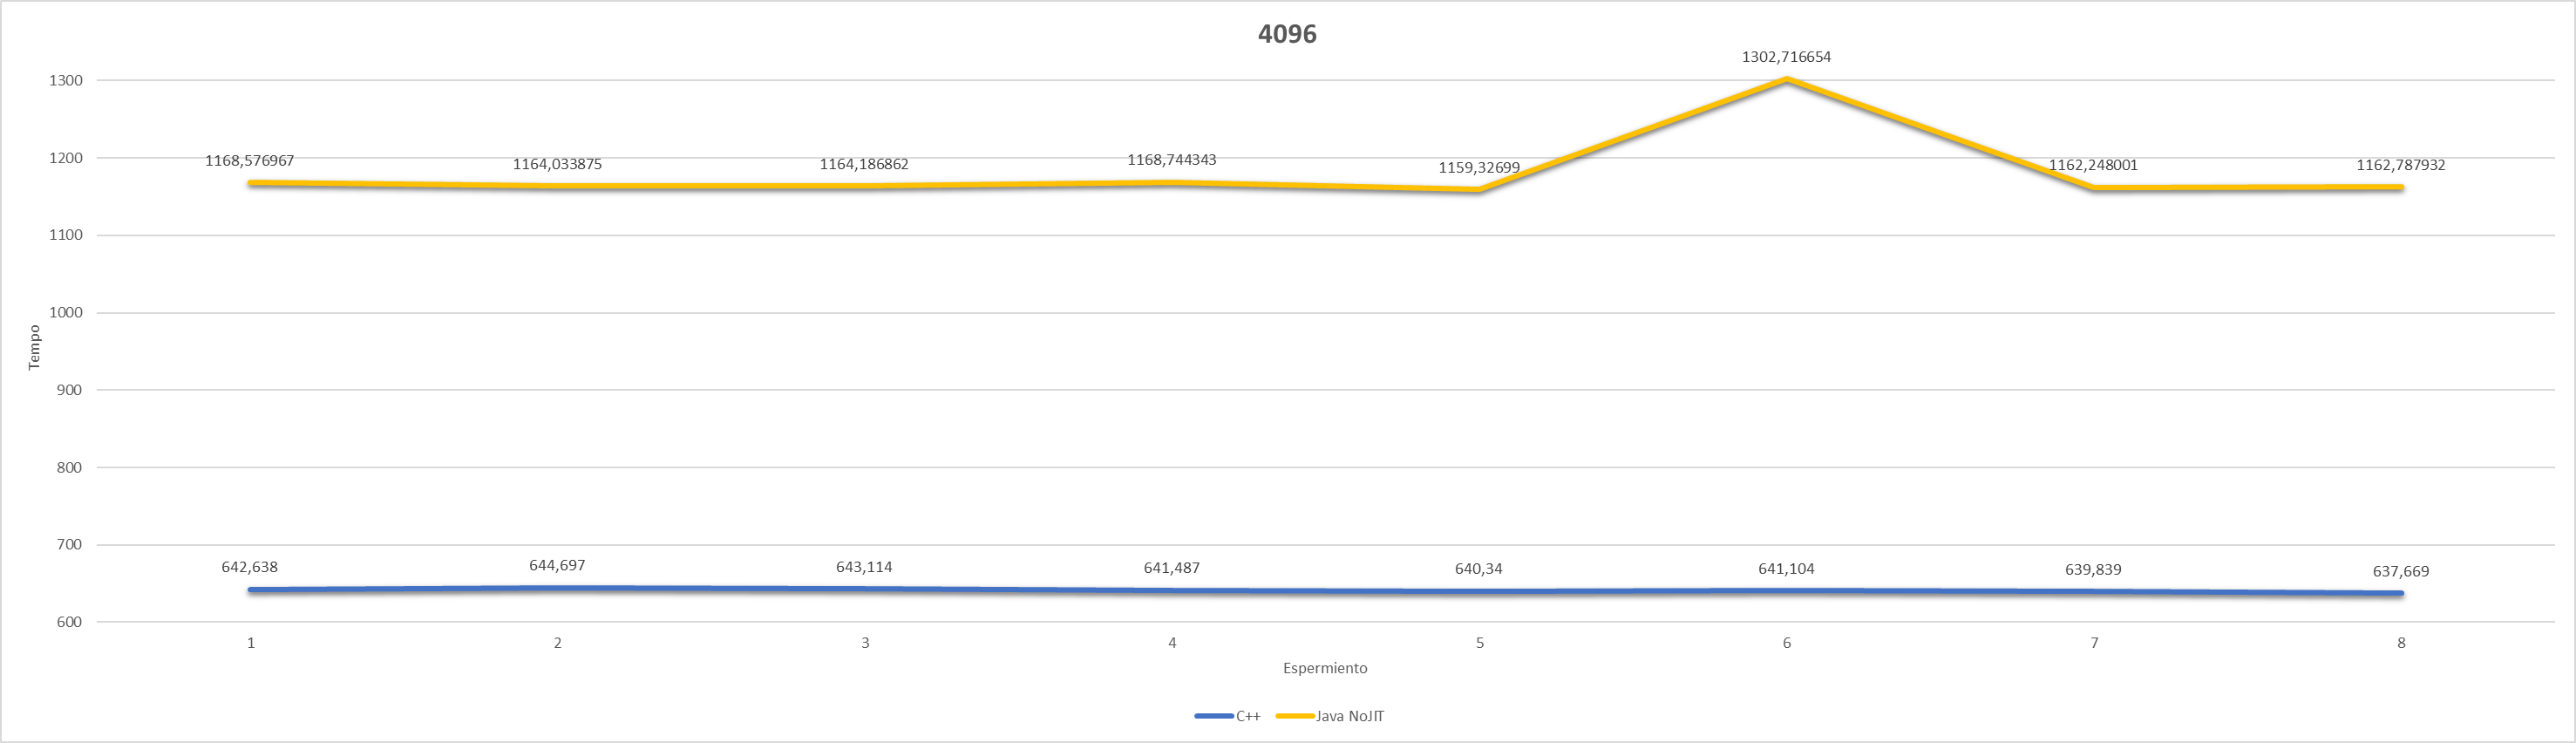
\includegraphics[width=1\linewidth,keepaspectratio]{grafico_tempi_4096_1}
  \caption{Confronto tempi \textbf{Java NoJIT} vs \textbf{C++} 4096x4096}
  \label{prodottomatrici_grafico_tempi_4096_1}
\end{figure}

Si noti che, per tutte le dimensioni considerate, Java con JIT e C++ O2 sono
molto più performanti delle corrispondenti versioni non ottimizzate.\\
\clearpage
\subsection{Significatività dei risultati}

Per verificare la significatività statistica delle 8 osservazioni fatte è fondamentale
dimostrare che le distribuzioni non siano statisticamente equivalenti, ovvero che
appartengano a popolazioni differenti.\\
A tal fine, la statistica inferenziale mette a disposizione diversi test(parametrici e non),
i quali possono essere applicati in modo opportuno solo conoscendo la natura
della distribuzione analizzata.\\
In particolare, è di interesse definire la normalità o meno dei dati che si hanno
a disposizione.\\
Per studiare la normalità della distribuzione si possono utilizzare i seguenti
parametri:

\begin{itemize}
  \item \textbf{Indice di Asimmetria}: cerca di fornire una misura sulla mancanza
  di simmetria in una distribuzione, il valore 0 è una condizione necessaria, ma
  non sufficiente, per la simmetria;
  \item \textbf{Curtosi}: fornisce una misura sull'appiattimento della curva,
  il valore dell'indice corrispondente ad una distribuzione normale è 0;
  \item \textbf{Coefficiente di Variazione}: permette di determinare la dispersione
  dei valori intorno alla media indipendentemente dall'unità di misura.
\end{itemize}

\'E possibile utilizzare, come test di verifica della normalità di una distribuzione,
il test di \textbf{Shapiro-Wilk} o test della bontà di adattamento.\\
Tale test restituisce il valore W, compreso nell’intervallo [0, 1], che per
valori vicini allo 0 indica una distribuzione \textbf{skewed}, mentre per valori
vicini ad 1 indica una distribuzione normale.\\
Un'ulteriore tecnica per la verifica della normalità dei dati prevede di
osservare il plot \textbf{Quantile-Quantile}, che presenta sull'asse delle ascisse
i valori tipici dei quantili di una normale, mentre sull'asse delle ordinate i
valori dei quantili della distribuzione osservata.\\
Questa tecnica visiva è molto robusta all'errore, e per questo motivo, molto usata.\\
L'interpretazione del plot Q-Q è abbastanza semplice: se i punti risultanti sono
difficilmente approssimabili con una retta, allora si può affermare, con buon
margine statistico, che è rifiutata l'ipotesi nulla che quella osservata sia una
distribuzione normale.\\
Viceversa, è possibile continuare a studiare con ulteriori parametri e test, la
normalità della distribuzione.\\

\clearpage

\subsubsection{Distribuzioni C++ O2}
Nella seguente figura sono riportate le distribuzioni, al crescere di N, del
linguaggio C++ con ottimizzazione O2 attiva.

\begin{figure}[!htbp]
  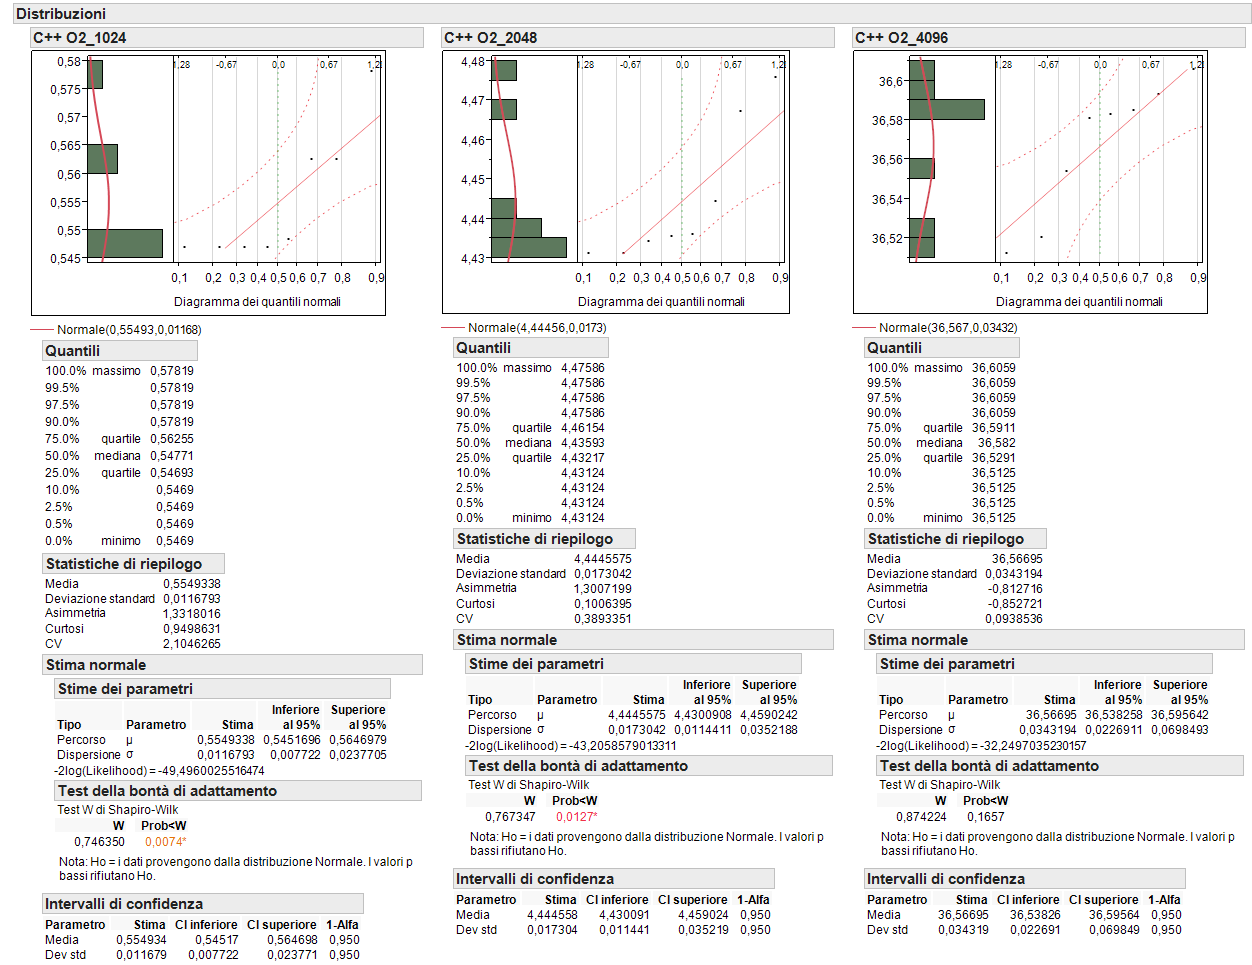
\includegraphics[width=1\linewidth,keepaspectratio]{distribuzione_cppO2}
  \caption{Distribuzioni osservazioni in C++ O2}
  \label{prodottomatrici_distribuzione_cppO2}
\end{figure}
Dalla \figurename~\ref{prodottomatrici_distribuzione_cppO2} si nota
che la distribuzione per dimensione 2048 non è normale poiché è rifiutata
l'ipotesi nulla del test Shapiro-Wilk, a differenza delle distribuzioni a 1024 e 4096,
in cui l'ipotesi nulla non è rigettata e quindi non è possibile affermare che
quella osservata non sia una normale.\\
Osservando il plot Q-Q si osserva che la distribuzione a 1024 non è approssimabile con una
retta e considerando anche gli indici di asimmetria e curtosi è possibile affermare che
la distribuzione è non normale, mentre per la distribuzione a 4096, anche se dal plot
Q-Q si potrebbe dire normale, osservando l'indice di curtosi è possibile rifiutare
la normalità.
\clearpage
\subsubsection{Distribuzioni C++ }
Nella seguente figura sono riportate le distribuzioni, al crescere di N, del
linguaggio C++.

\begin{figure}[!htbp]
  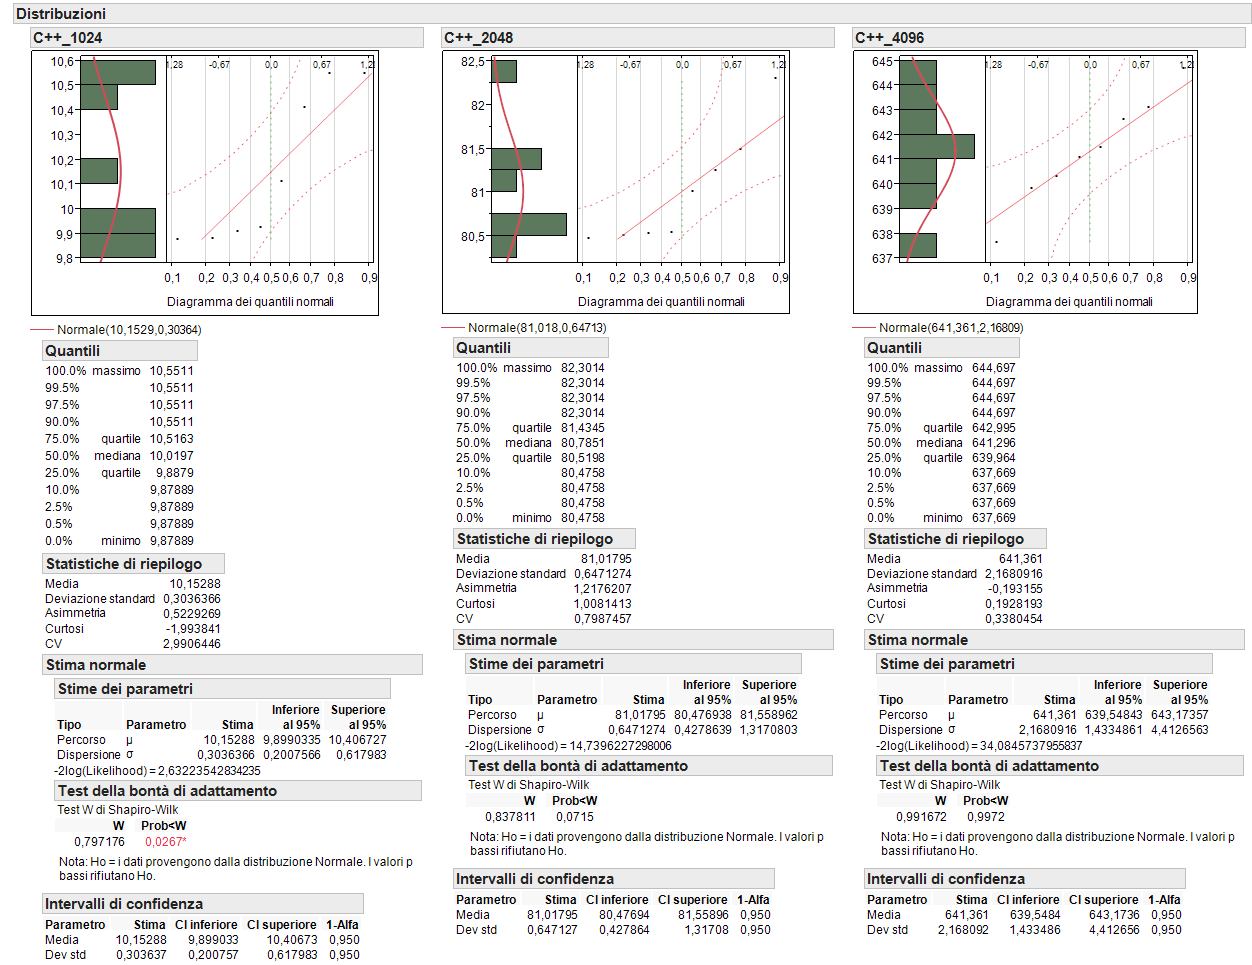
\includegraphics[width=1\linewidth,keepaspectratio]{distribuzione_cpp}
  \caption{Distribuzioni osservazioni in C++}
  \label{prodottomatrici_distribuzione_cpp}
\end{figure}

Dalla \figurename~\ref{prodottomatrici_distribuzione_cpp} si nota
che le distribuzioni per dimensioni 1024 e 4096 non sono normali poiché è rifiutata
l'ipotesi nulla del test Shapiro-Wilk, a differenza della distribuzione 2048,
in cui l'ipotesi nulla non è rigettata e quindi non è possibile affermare
che quella osservata non sia una normale.\\
Osservando il plot Q-Q si osserva che la distribuzione con N pari a 2048 è approssimabile con una
retta e considerando anche gli indici di asimmetria e curtosi è possibile osservare che
la distribuzione sia normale.\\
\clearpage
\subsubsection{Distribuzioni Java}
Nella seguente figura sono riportate le distribuzioni, al crescere di N, del
linguaggio Java.

\begin{figure}[!htbp]
  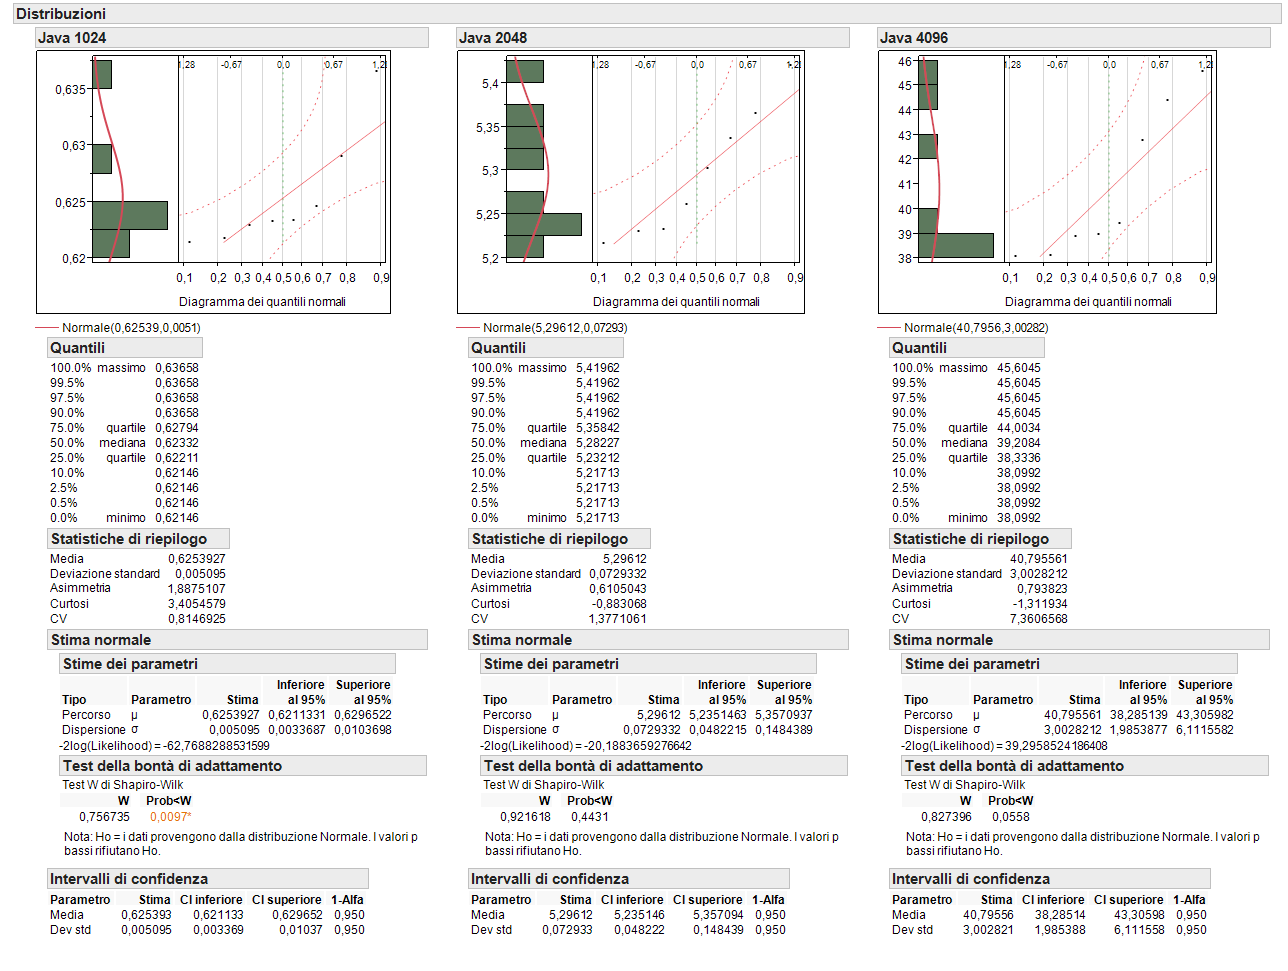
\includegraphics[width=1\linewidth,keepaspectratio]{distribuzione_java}
  \caption{Distribuzioni osservazioni in Java}
  \label{prodottomatrici_distribuzione_java}
\end{figure}

Dalla \figurename~\ref{prodottomatrici_distribuzione_java} si nota
che la distribuzione per dimensione 1024 non è normale, essendo rifiutata
l'ipotesi nulla del test Shapiro-Wilk, a differenza delle distribuzioni 2048 e
4096, in cui l'ipotesi nulla non è rigettata e quindi non è possibile affermare
che quella osservata non sia una normale.\\
Osservando il plot Q-Q si osserva che la distribuzione con N pari a 2048
è approssimabile con una retta, e considerando anche l'indice di asimmetria
e di curtosi è possibile osservare che la distribuzione sia normale, mentre
per la distribuzione con N pari a 4096 è possibile rigettare l'ipotesi di normalità.\\

\clearpage
\subsubsection{Distribuzioni Java No JIT}
Nella seguente figura sono riportate le distribuzioni, al crescere di N, del
linguaggio Java con JIT Compiler disattivato.

\begin{figure}[!htbp]
  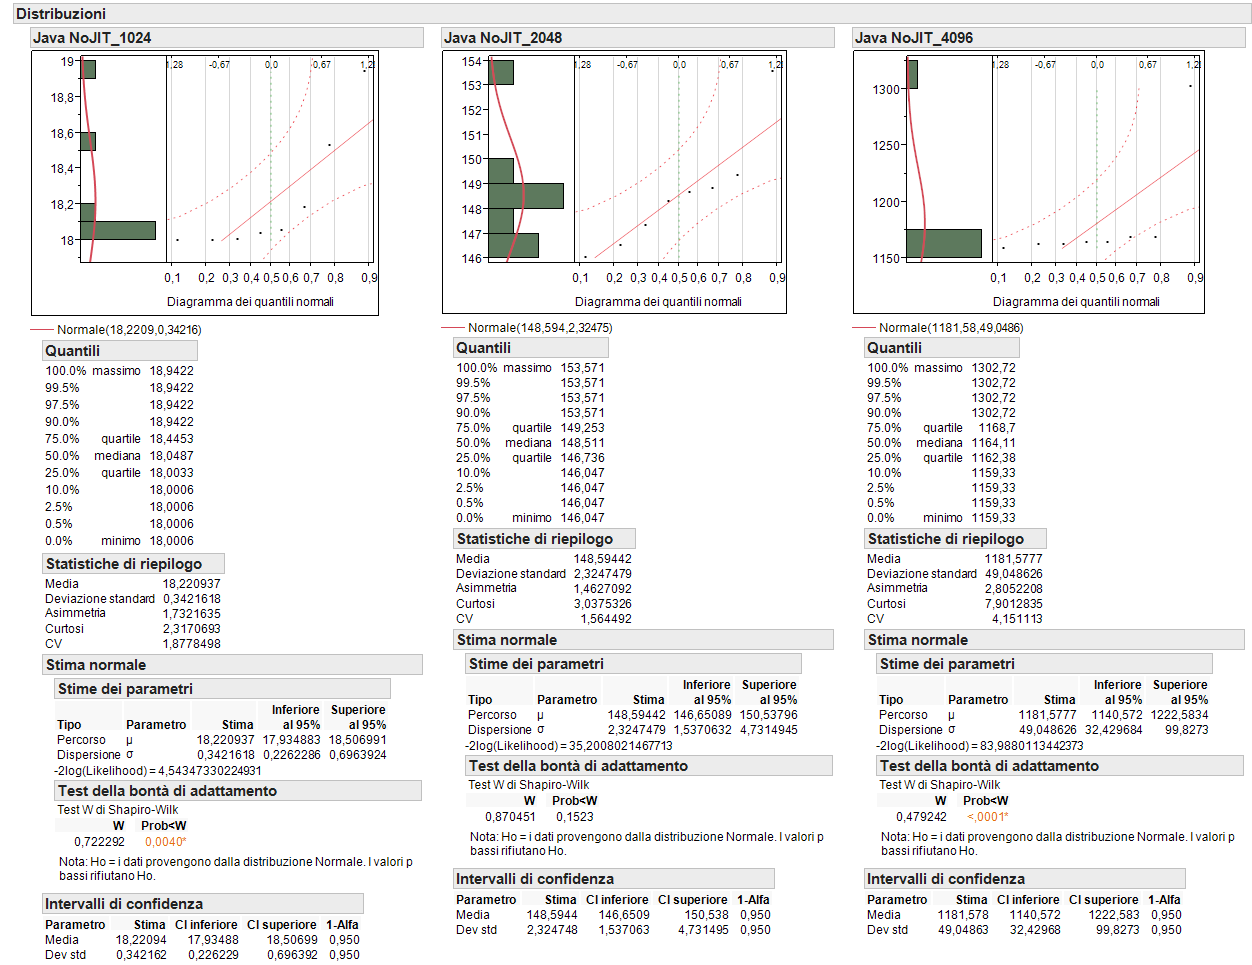
\includegraphics[width=1\linewidth,keepaspectratio]{distribuzione_javaNoJIT}
  \caption{Distribuzioni osservazioni in Java NoJIT}
  \label{prodottomatrici_distribuzione_javaNoJIT}
\end{figure}

Dalla \figurename~\ref{prodottomatrici_distribuzione_javaNoJIT} si nota
che le distribuzioni per dimensione pari a 1024 e 2048 non sono normali, essendo
rifiutata l'ipotesi nulla del test Shapiro-Wilk, a differenza della distribuzione
4096, in cui l'ipotesi nulla non è rigettata e quindi non è possibile affermare
che quella osservata non sia una normale.\\
Osservando il plot Q-Q si osserva che la distribuzione con N pari a 4096 è
approssimabile con una retta e considerando gli indici di asimmetria e di
curtosi è possibile affermare che la distribuzione è normale.\\

\clearpage
\subsubsection{Intervallo di confidenza}
Un’ultima osservazione da dover fare riguarda gli intervalli di confidenza ottenuti in
analisi preliminare.\\
A causa della non normalità della maggioranza delle distribuzioni, si è deciso di
utilizzare la mediana come indice di tendenza centrale. \\
Confrontando le mediane delle distribuzioni dei campioni
con gli intervalli di confidenza ottenuti in analisi preliminare si nota che non
tutte le distribuzioni rispettano le ipotesi fatte.\\ Questo significa che l’ipotesi
di normalità sostenuta nella fase preliminare, per alcune delle distribuzioni,
potrebbe venir meno.\\
Di seguito è riportata una tabella che riassume gli intervalli di confidenza
ottenuti in analisi preliminare e le mediane ottenute dai campioni raccolti
successivamente.

\begin{figure}[!htbp]
  \centering
  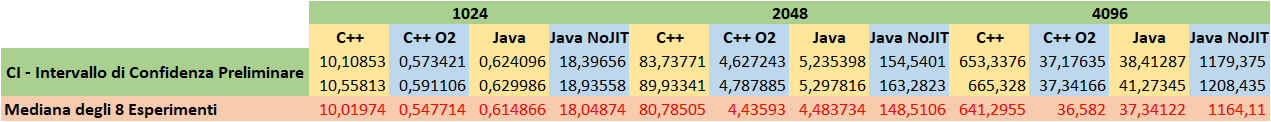
\includegraphics[width=1\linewidth,keepaspectratio]{CI_mediana}
  \caption{Intervalli di confidenza}
  \label{prodottomatrici_CI_mediana}
\end{figure}

Come si può osservare, che non tutte le medie calcolata sugli 8 esperimenti finali
rientrano nell'intervallo di confidenza calcolato sugli esperimenti effettuati
in fase preliminare.\\

\clearpage
\subsection{Validazione campioni}
Come detto in precedenza, si è deciso di utilizzare la mediana come indice di
tendenza centrale.\\
Per verificare la significatività dei campioni non è possibile applicare il
\textbf{T-Test}(valido nel caso in cui i campioni appartengono ad una Normale),
ma bisogna affidarsi a test non parametrici come il test di
\textbf{Wilcoxon/Kruskal-Wallis}.\\
Il test di Kruskal-Wallis, in particolare, serve a verificare se 2 o più campioni
indipendenti appartengono alla stessa popolazione.\\
Di seguito vengono mostrati i risultati ottenuti da JMP.\\

\begin{figure}[!htbp]
  \centering
  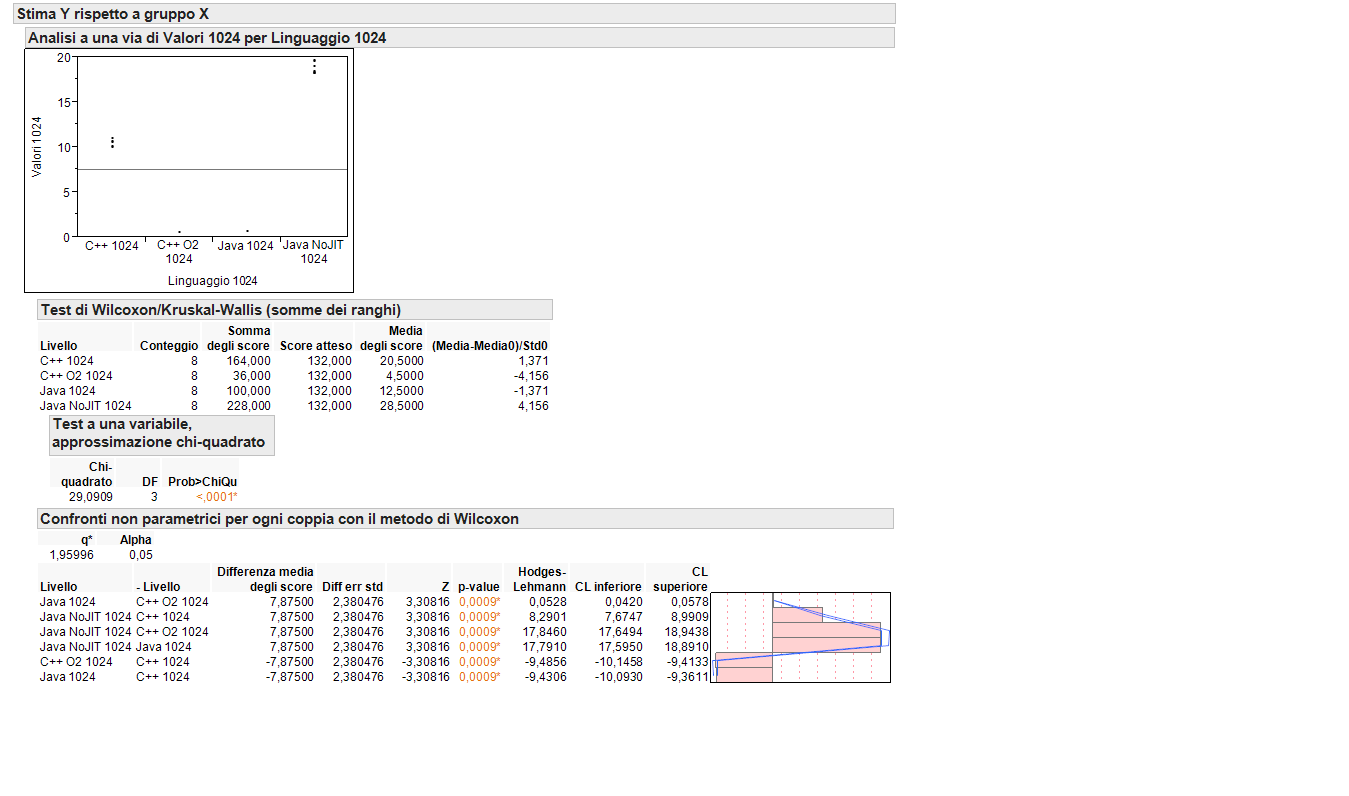
\includegraphics[width=1\linewidth,keepaspectratio]{Wilcoxon_Kruskal-Wallis_1024}
  \caption{Test di Wilcoxon/Kruskal-Wallis con matrici quadrate di dimensione 1024}
  \label{prodottomatrici_Wilcoxon_Kruskal-Wallis_1024}
\end{figure}

\clearpage

\begin{figure}[!htbp]
  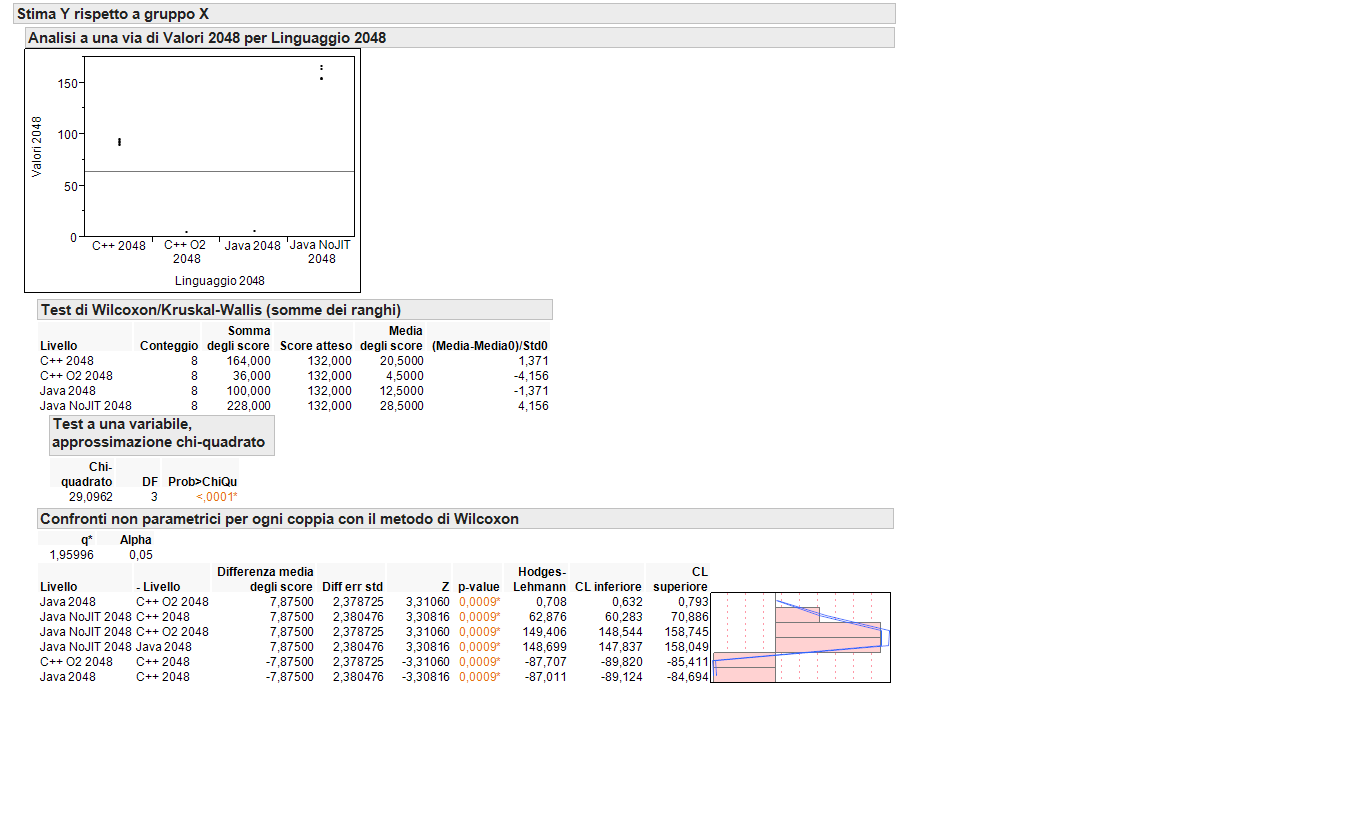
\includegraphics[width=1\linewidth,keepaspectratio]{Wilcoxon_Kruskal-Wallis_2048}
  \caption{Test di Wilcoxon/Kruskal-Wallis con matrici quadrate di dimensione 2048}
  \label{prodottomatrici_Wilcoxon_Kruskal-Wallis_2048}
\end{figure}

\clearpage

\begin{figure}[!htbp]
  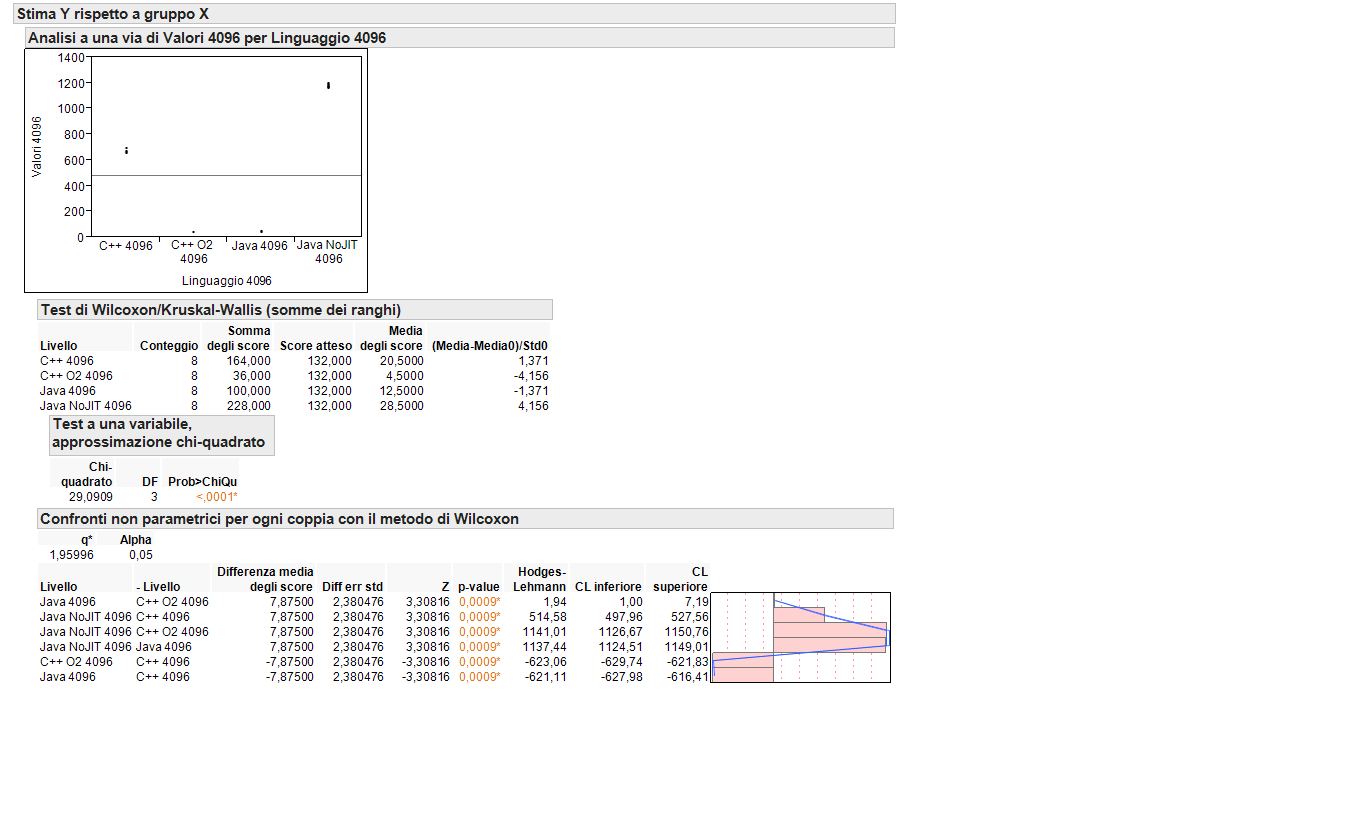
\includegraphics[width=1\linewidth,keepaspectratio]{Wilcoxon_Kruskal-Wallis_4096}
  \caption{Test di Wilcoxon/Kruskal-Wallis con matrici quadrate di dimensione 4096}
  \label{prodottomatrici_Wilcoxon_Kruskal-Wallis_4096}
\end{figure}

Tutti i test hanno portato alla stessa conclusione: l'ipotesi nulla è
rifiutata ($pvalue < 0.05$), di conseguenza i differenti gruppi non appartengono
alla stessa popolazione.\\

\clearpage

\section{Conclusioni}
Se si utilizzano ottimizzazioni configurabili dal compiler, in particolare O2
per C++ e il JIT in Java, il linguaggio di programmazione C++ risulta essere il
più veloce.\\
Tuttavia, disattivando ogni ottimizzazione dei compiler, il linguaggio C++
risulta essere comunque migliore di Java.\\
La supremazia del C++ discende dal fatto che è un linguaggio compilato ed
eseguito direttamente sulla macchina fisica, mentre il linguaggio Java è compilato
per ottenere un bytecode e poi interpretato ed eseguito sulla JVM, a sua volta
eseguita sulla macchina fisica.

\subsection{C++}
\subsubsection{Main}
\lstinputlisting[language=C++, caption={Codice C++}]{main.cpp}

\subsection{Java}
\subsubsection{MatrixMultiplicationù Class}
\lstinputlisting[language=Java, caption={Codice Java}]{MatrixMultiplication.java}
\subsubsection{Main}
\lstinputlisting[language=Java, caption={Codice Java}]{testMatrix.java}

\clearpage

\section{Script Batch}
Script per l'automazione degli esperimenti, al variare della
dimensione N, per tutti e quattro i casi(C++, Java, C++ O2, Java NoJIT).\\
\lstinputlisting[language=command.com, caption={Script Batch}]{script.bat}

\clearpage
Script per l'esecuzione nel particolare linguaggio scelto, per un numero
designato di volte, dell'algoritmo di Prodotto Matriciale.\\
\subsubsection{C++}
\lstinputlisting[language=command.com, caption={Script Batch}]{script_strassen_cpp.bat}
\subsubsection{Java}
\lstinputlisting[language=command.com, caption={Script Batch}]{script_strassen_java.bat}

	% !TEX root = ./main.tex
% !TEX encoding = UTF-8 Unicode
% !TEX program = pdflatex
% !TeX spellcheck = it_IT

\graphicspath{{Immagini/},{Immagini/pca_clustering/}}

\chapter{PCA \& Clustering}
Estrapolare un Workload sintetico a partire dal workload reale, riportato nel file
 \textit{PCA-CLASTERING-2017.jmp}.

\section{Obiettivo}
A partire dal workload reale, si vuole ottenere un \textbf{workload sintetico},
caratterizzato da un numero di osservazioni minori, che conservi quanta
più varianza possibile.

\section{Estrazione del Workload Sintetico}
Per estrarre il workload sintetico, dopo aver visionato i dati, si è scelto
di seguire il seguente procedimento:

\begin{itemize}
  \item Analisi del \textbf{\textit{CV(Coefficiente di Variazione)}}, per
  eliminare i parametri statisticamente non significativi;
  \item \textbf{\textit{PCA(Principal Component Analysis)}}, per ridurre il
  numero di parametri ed eliminare la correlazione tra essi;
  \item \textbf{\textit{Clustering}}, per ridurre il numero di esperimenti.
\end{itemize}


\subsection{Analisi del Coefficiente di Variazione}
In prima istanza, è stata effettuata un'analisi sul coefficiente di variazione(CV),
il quale esprime la dispersione dei valori dei singoli parametri attorno alla loro media.\\
Quando il coefficiente di variazione è nullo, il parametro
corrispondente non è statisticamente significativo e quindi è possibile eliminarlo.\\
Nella \figurename~\ref{cv} si evince l'assenza di colonne con coefficiente di variazione nullo,
quindi tutti i parametri dovranno essere utilizzati nelle successive fasi di analisi.

\begin{figure}[!htbp]
  \centering
	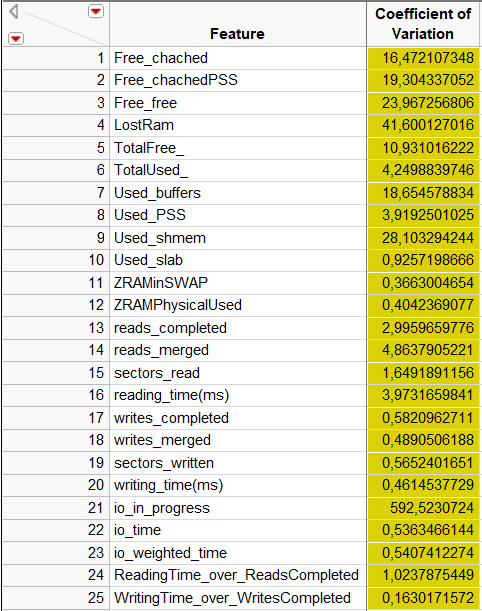
\includegraphics[width=.7\linewidth,keepaspectratio]{cov.png}
  \caption{Coefficiente di Variazione(CV)}
  \label{cv}
\end{figure}
\clearpage

\subsection{PCA}
In questa fase è stata applicata la
\textbf{\textit{PCA(Principal Component Analysis)}},
la quale trasforma un workload con parametri correlati in uno contenente parametri
incorrelati, ottenuti come combinazione lineare, pesata, di quelli iniziali.\\
L'utilizzo della PCA è fondamentale anche per la successiva fase di clustering, in
quanto quest'ultimo necessita che sia rispettata la proprietà di incorrelazione
dei parametri.\\
Per effettuare la PCA si è fatto utilizzo del tool statistico \textit{\textbf{JMP}}, nella
\figurename~\ref{pca} è riportato l'output.\\

\begin{figure}[!htbp]
	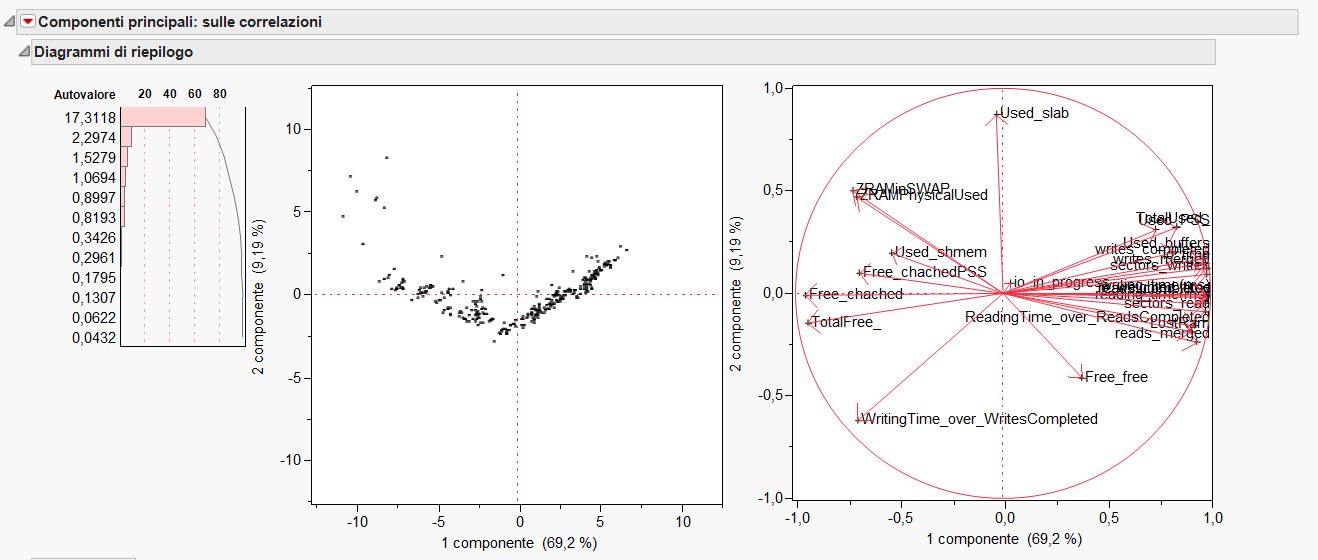
\includegraphics[width=\linewidth,keepaspectratio]{pca.png}
  \caption{Risultato PCA}
  \label{pca}
\end{figure}

\clearpage

Nella \figurename~\ref{autovalori} sono riportati gli autovalori ottenuti dalla PCA.\\

\begin{figure}[!htbp]
	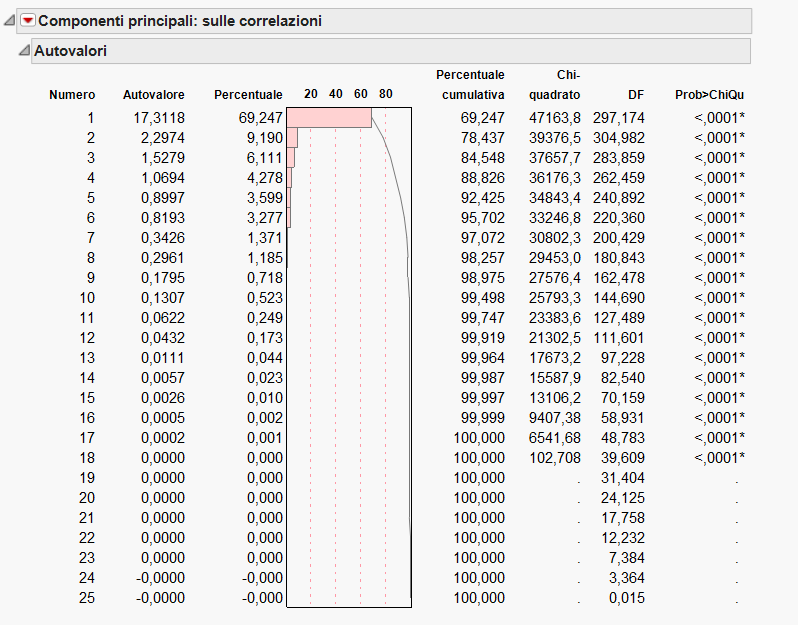
\includegraphics[width=\linewidth,keepaspectratio]{autovalori.png}
  \caption{Autovalori PCA}
  \label{autovalori}
\end{figure}

\clearpage

\begin{figure}[!htbp]
	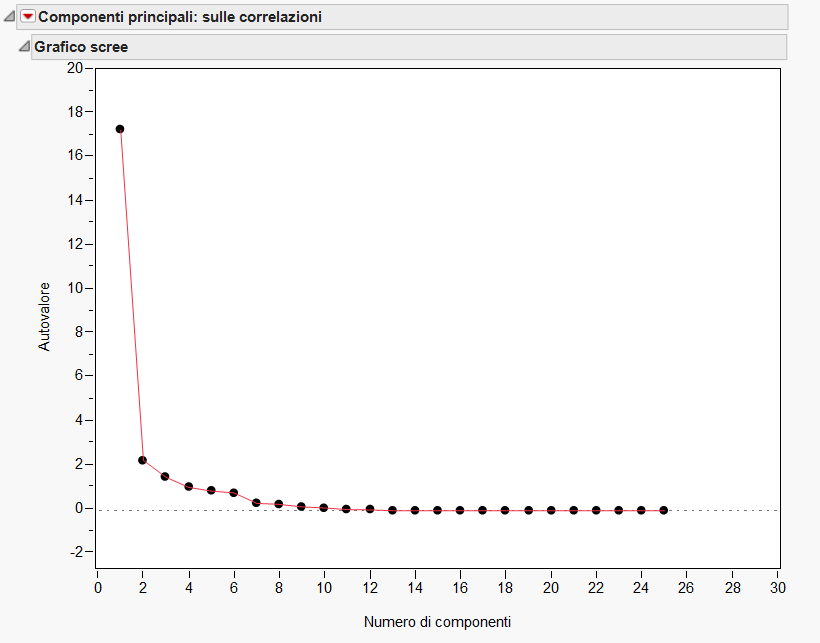
\includegraphics[width=\linewidth,keepaspectratio]{grafico_scree.png}
  \caption{Grafico Scree}
  \label{grafico_scree}
\end{figure}

\'E possibile scegliere il numero di componenti principali da utilizzare considerando
il ginocchio della curva ottenuta nella \figurename~\ref{grafico_scree}, rappresentante
sull'asse x il numero di componenti principali e sull'asse y
gli autovalori.\\
In questo caso, scegliendo di considerare 6 componenti principali, si è sicuri di conservare una quota di varianza sufficientemente
significativa(\textit{95,703\%}).\\
\clearpage
\begin{figure}[!htbp]
	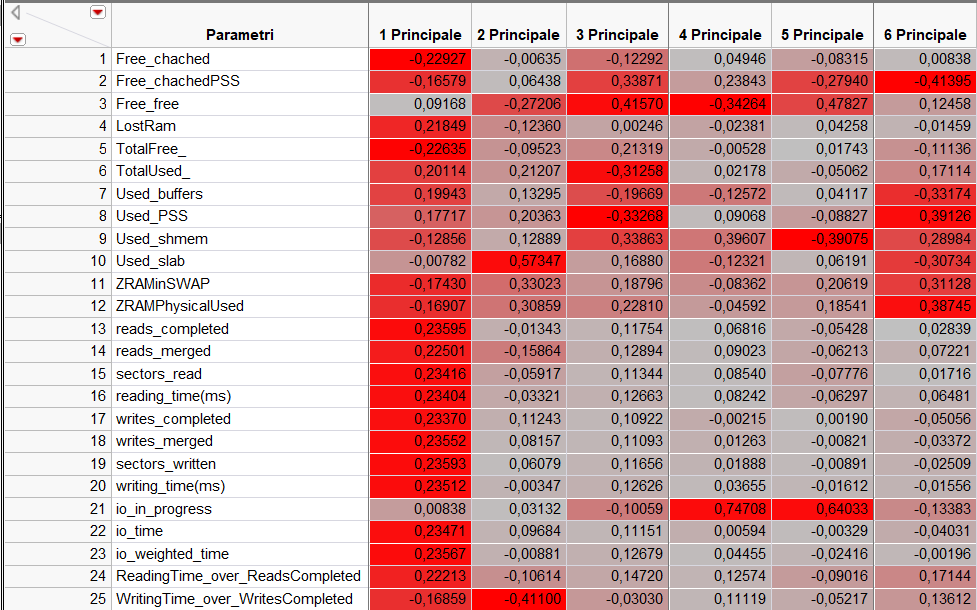
\includegraphics[width=\linewidth,keepaspectratio]{autovettori.png}
  \caption{Autovettori}
  \label{autovettori}
\end{figure}

Nella \figurename~\ref{autovettori} sono sfumati in rosso i parametri che
hanno contribuito maggiormente, in segno positivo o negativo, alla creazione
delle componenti principali scelte.\\
Valori vicini allo 0 indicano che quei parametri pesano relativamente poco nel
calcolo della componente principale.\\

% In particolare:
% \begin{itemize}
%   \item \textbf{\textit{Principale 1:}} \textit{Free\_chached, LostRam, TotalFree,
%   reads\_completed, reads\_merged, sectors\_read, reading\_time(ms),
%   writes\_completed, writes\_merged, sector\_written, writing\_time(ms),
%   io\_time, io\_weighted\_time e ReadingTime\_over\_ReadsCompleted};
%   \item \textbf{\textit{Principale 2:}} \textit{Used\_slab e WritingTime\_over\_WritesCompleted};
%   \item \textbf{\textit{Principale 3:}} \textit{Free\_free, TotalUsed e Used\_PSS};
%   \item \textbf{\textit{Principale 4:}} \textit{io\_in\_progress};
%   \item \textbf{\textit{Principale 5:}} \textit{Used\_shmem};autovettori
%   \item \textbf{\textit{Principale 6:}} \textit{Free\_chachedPSS, Used\_buffers e Used\_PSS, ZRamPhysicalUsed};
% \end{itemize}
\clearpage
\subsection{Clustering}
In questa fase è stato effettuata un'operazione di clustering sul risultato
ottenuto dallo step precedente.\\
La tecnica di clusterizzazione scelta è di tipo gerarchico agglomerativo,
in particolare è stata utilizzata la metrica di \textbf{Ward} per l'aggregazione
dei cluster.\\
Il criterio di Ward è diretto alla minimizzazione della varianza all’interno dei gruppi,
pertanto si presta bene ad essere utilizzato con variabili quantitative.\\
In \figurename~\ref{dendogramma} è riportato il dendogramma risultante.\\

\begin{figure}[!htbp]
	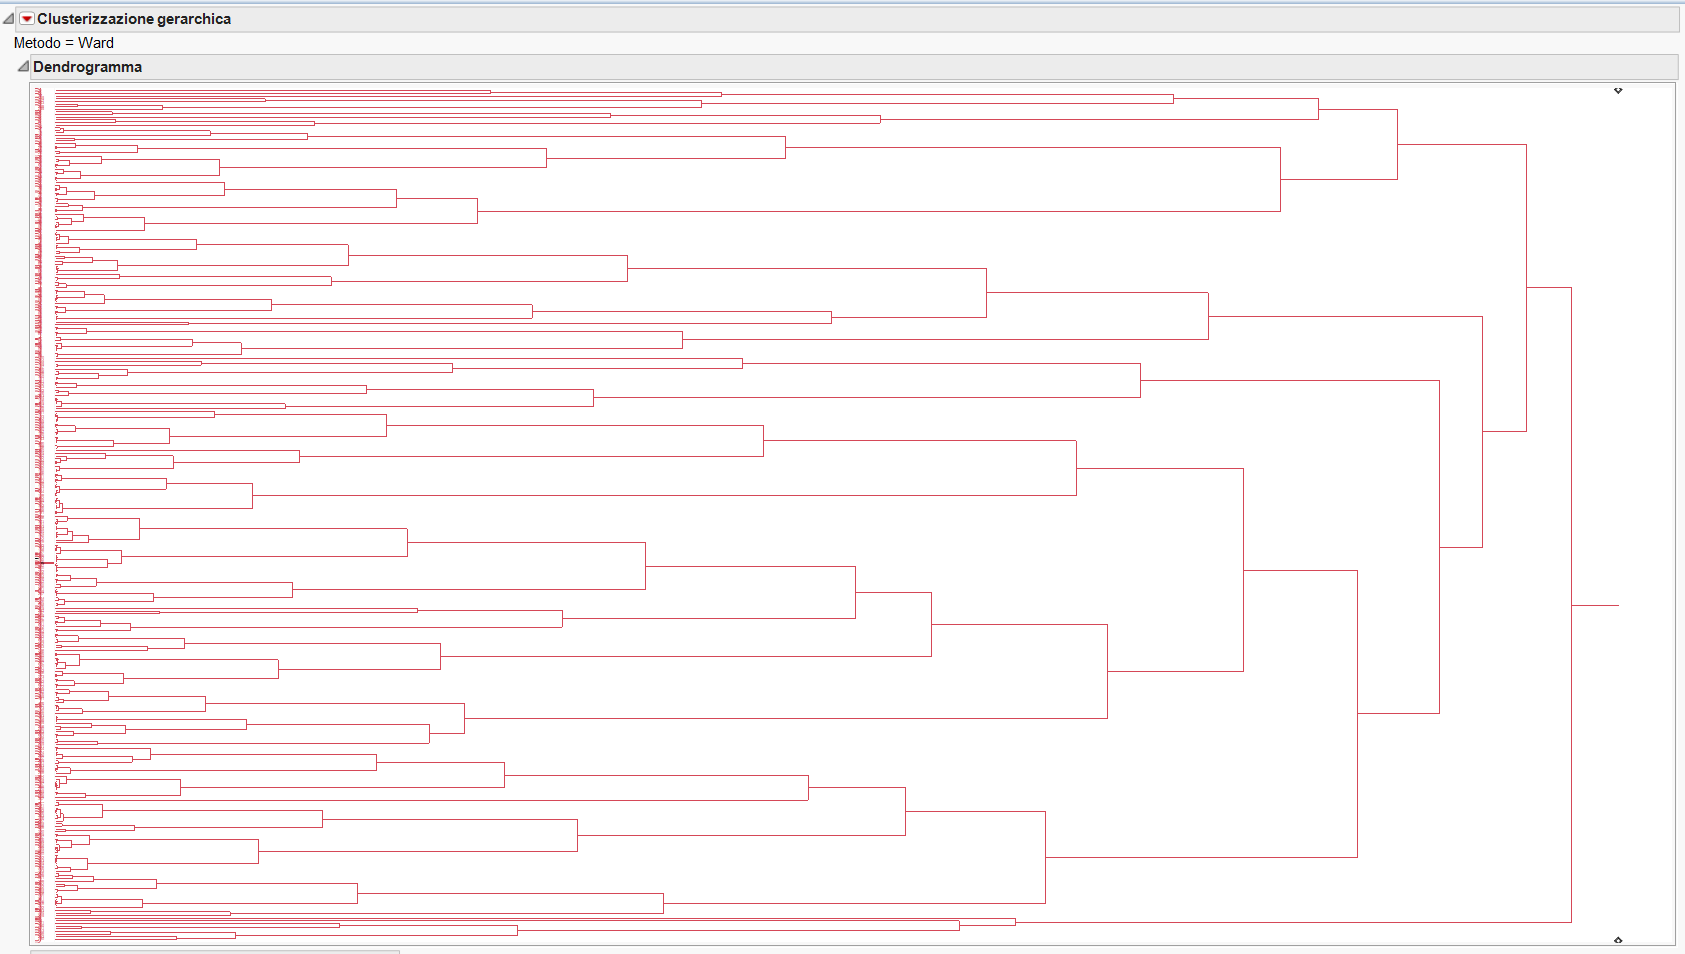
\includegraphics[width=\linewidth,keepaspectratio]{dendogramma.png}
  \caption{Dendogramma}
  \label{dendogramma}
\end{figure}
\clearpage
\begin{figure}[!htbp]
	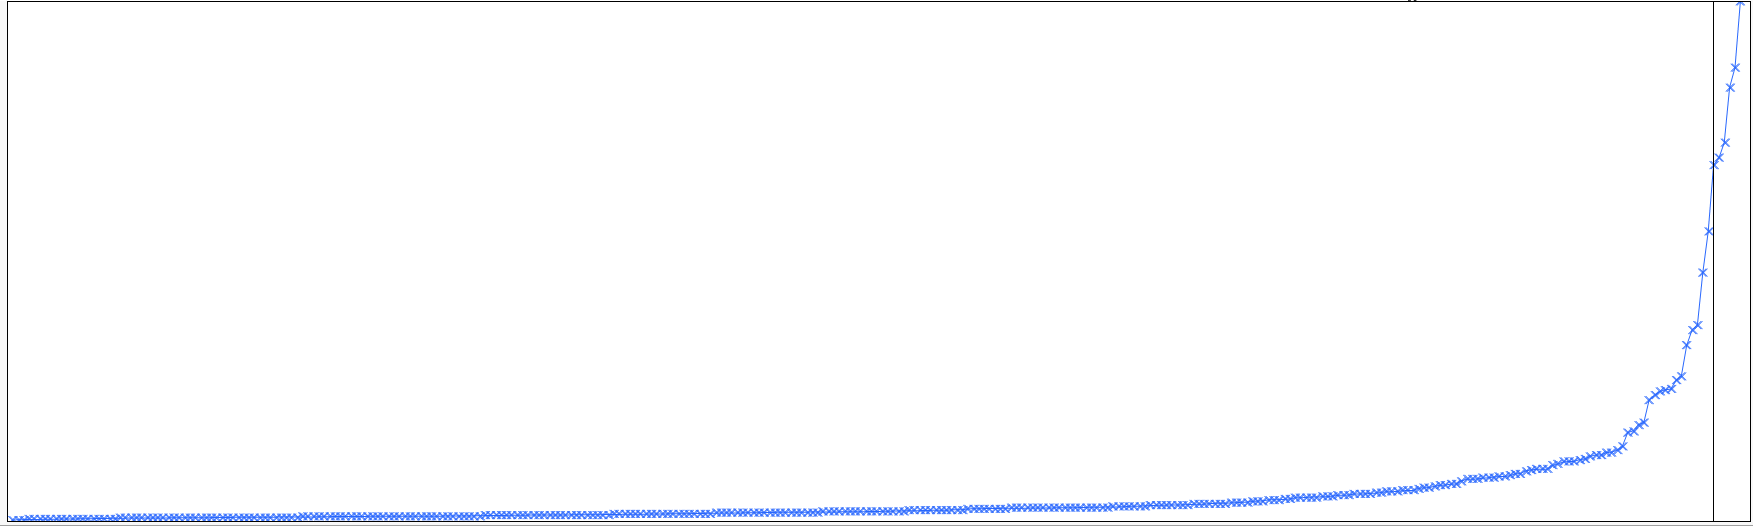
\includegraphics[width=\linewidth,keepaspectratio]{curva_dendogramma.png}
  \caption{Curva di Clustering}
  \label{curva_dendogramma}
\end{figure}

Facendo riferimento alla \figurename~\ref{curva_dendogramma}, è possibile scegliere
il numero di cluster posizionandosi nel ginocchio della curva, rappresentante le
distanze tra cluster.\\
In maniera analoga si può scegliere il numero di cluster utilizzando il criterio
di clusterizzazione cubica(\textbf{CCC}), riportato in \figurename~\ref{ccc},
scegliendo il numero di cluster in funzione della regola del massimo salto.\\

\begin{figure}[htbp]
\centering
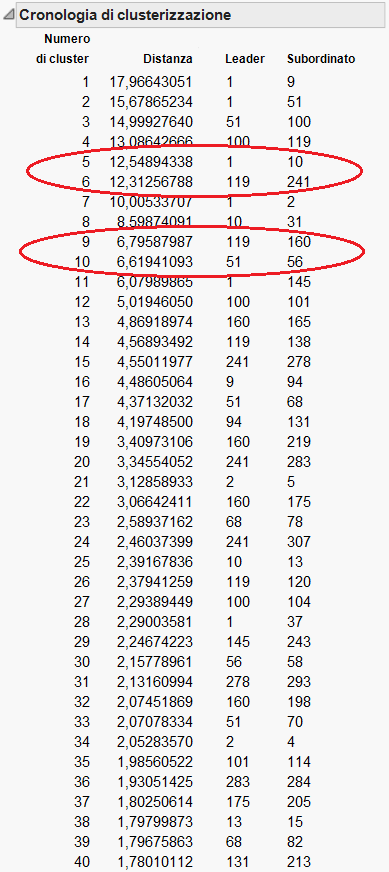
\includegraphics[width=50mm]{gerarchia_clustering.png}% "%" necessario
\qquad\qquad
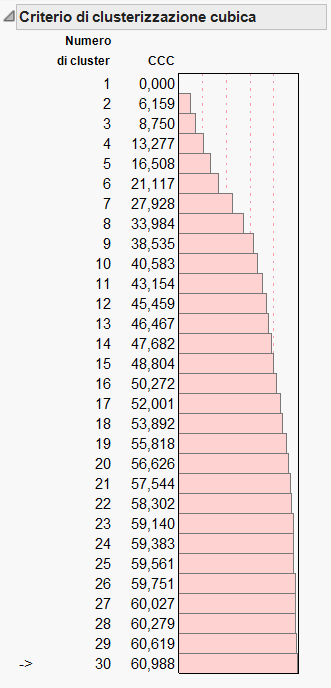
\includegraphics[width=50mm]{ccc.png}
\caption{Gerarchia Clustering e Criterio di Clusterizzazione Cubica}
\label{ccc}
\end{figure}

\clearpage

Sulla base dei criteri illustrati, si è scelto di considerare due soluzioni:
5 e 9 cluster.\\
Per generare i workload sintetici, inoltre, si è scelto di considerare il
centroide di ogni cluster.\\

\begin{figure}[!htbp]
	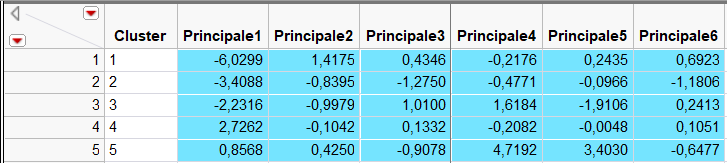
\includegraphics[width=\linewidth,keepaspectratio]{centroidi(5).png}
  \caption{Workload sintetico ottenuto con 5 cluster}
  \label{}
\end{figure}

\begin{figure}[!htbp]
	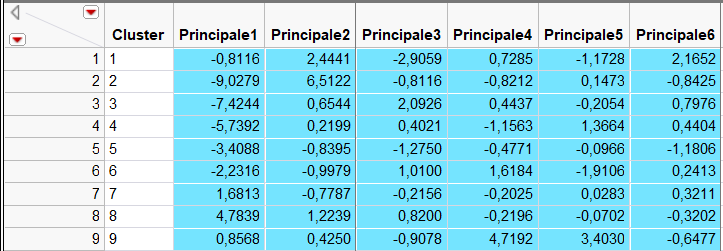
\includegraphics[width=\linewidth,keepaspectratio]{centroidi(9).png}
  \caption{Workload sintetico ottenuto con 9 cluster}
  \label{centroidi9}
\end{figure}

\clearpage
\section{Analisi}
Ottenuti i Workload Sintetici, è fondamentale osservare quanta varianza si è
conservata.\\
Per capire se la soluzione a 9 cluster è più conveniente della soluzione
a 5 cluster, bisogna confrontare la significatività conservata dai due workload sintetici.\\
Per fare ciò bisogna calcolare la varianza persa in ogni fase del processo di
caratterizzazione.\\
A valle della PCA, scegliendo solo 6 componenti principali, la varianza conservata
 risulta essere il 95,702\% della totale(valore ottenuto in JMP).\\
Per definire la significatività dei workload ottenuti con il clustering, invece, bisogna
utilizzare la devianza.\\
Quest'ultima è una grandezza indipendente dal grado di libertà, quindi si presta
perfettamente all'uso con i cluster, i quali hanno cardinalità differente.\\

La devianza del clustering è calcolata come la somma della devianza \textbf{inter-cluster}
e \textbf{intra-cluster}.\\
Tipicamente, per effettuare un buon clustering, si cerca di massimizzare la varianza
inter-clustering e minimizzare quella intra-clustering.\\
Nella seguente figura è riportata la devianza del workload sottoposto a PCA.\\

\begin{figure}[!htbp]
  \centering
	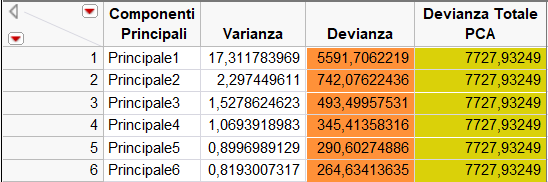
\includegraphics[width=.7\linewidth,keepaspectratio]{devianza_pca.png}
  \caption{Devianza PCA}
  \label{}
\end{figure}
\clearpage

\subsubsection{5 cluster}

Nella seguente figura è riportata la devianza inter-cluster.\\

\begin{figure}[!htbp]
  \centering
	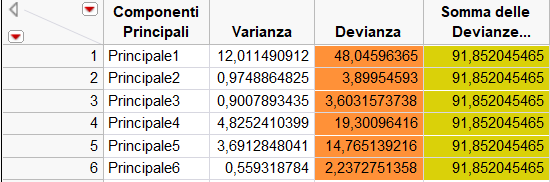
\includegraphics[width=.7\linewidth,keepaspectratio]{devianza_inter_clusters(5).png}
  \caption{Devianza Inter-Cluster}
  \label{}
\end{figure}

Nella seguente figura è riportata la devianza intra-cluster.\\

\begin{figure}[!htbp]
  \centering
	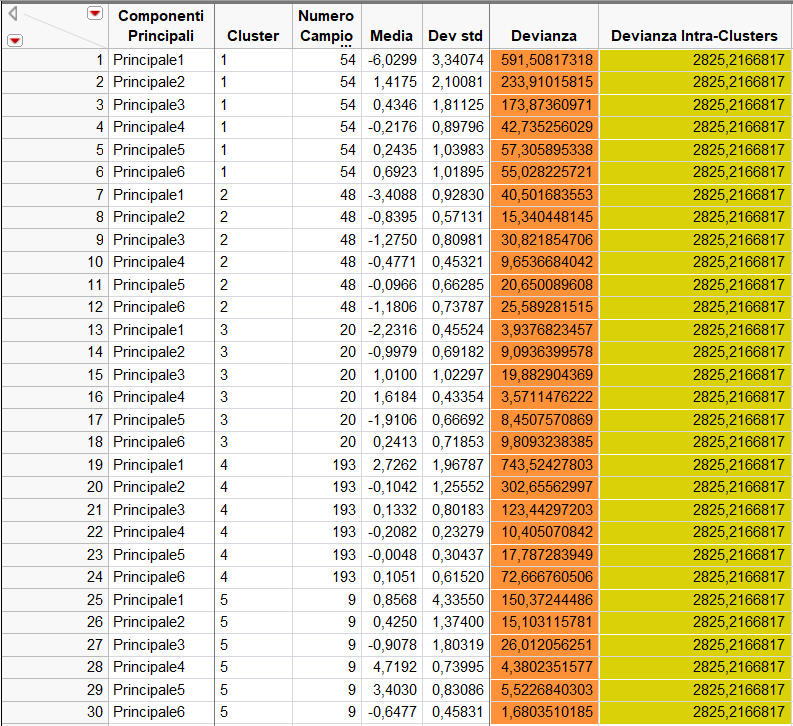
\includegraphics[width=.7\linewidth,keepaspectratio]{devianza_intra_clusters(5).png}
  \caption{Devianza Intra-Cluster}
  \label{}
\end{figure}
\clearpage

\subsubsection{9 cluster}

Nella seguente figura è riportata la devianza inter-cluster.\\

\begin{figure}[!htbp]
  \centering
	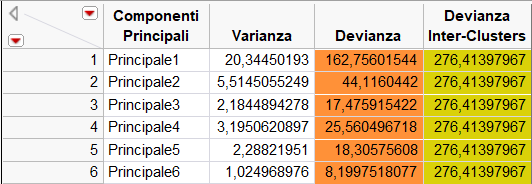
\includegraphics[width=.7\linewidth,keepaspectratio]{devianza_inter_clusters(9).png}
  \caption{Devianza Inter-Cluster}
  \label{}
\end{figure}

Nella seguente figura è riportata la devianza intra-cluster.\\

\begin{figure}[!htbp]
  \centering
	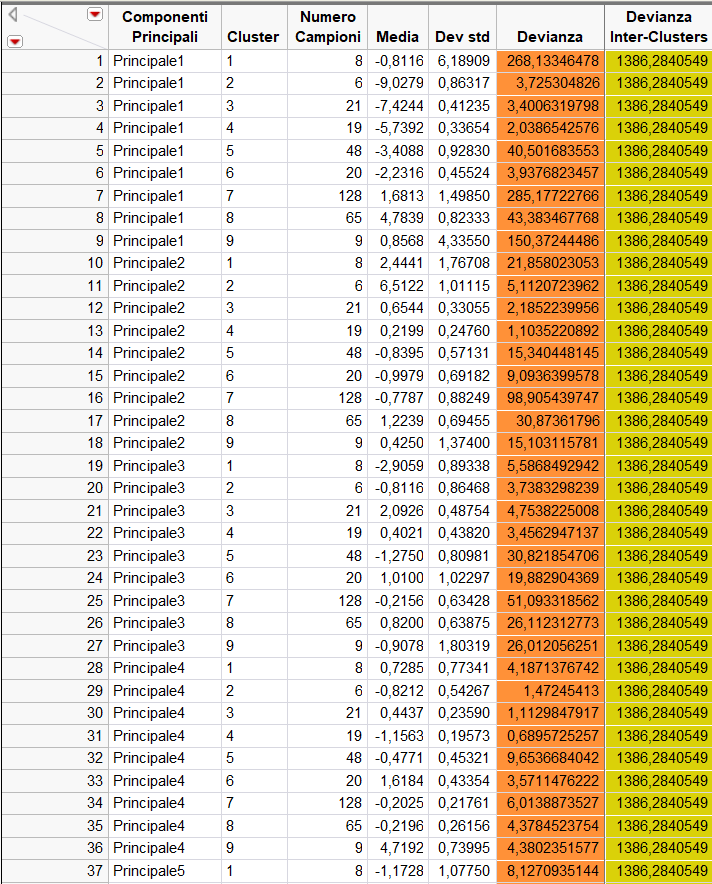
\includegraphics[width=.5\linewidth,keepaspectratio]{devianza_intra_clusters(9).png}
  \caption{Devianza Intra-Cluster}
  \label{}
\end{figure}
\clearpage
\section{Conclusioni}

Dopo aver ottenuto i valori di devianza del workload sottoposto a PCA e, successivamente,
a Clustering, considerando 5 e 9 cluster, è possibile calcolarne la significatività.\\
La devianza conservata utilizzando la tecnica di clustering si calcola con la
seguente formula:
$$1-{devianza_{inter\_cluster}+devianza_{intra\_cluster}\over {devianza_{pca}}}$$

Nelle seguenti Tabelle sono riportate le percentuali di devianza persa e conservata,
 nei due casi analizzati.\\
\vspace{5 mm}

\begin{center}
  \textbf{5 Cluster}
\end{center}
\begin{figure}[!htbp]
  \centering
  \begin{tabular}{|c|c|}
  \hline
  \textbf{Devianza PCA}	& 7727,93249 \\
  \hline
  \textbf{Devianza Clustering(intra-cluster+inter-cluster)}	& 2917,0687 \\
  \hline
  \textbf{Percentuale devianza persa con il clustering}	& 37,75\% \\
  \hline
  \textbf{Percentuale devianza conservata con il clustering}	& 62,25\% \\
  \hline
  \textbf{Significatività PCA} &	95,70\% \\
  \hline
  \end{tabular}
  %\caption{Workload con 5 cluster}
\end{figure}


\vspace{5 mm}
\begin{center}
  \textbf{9 Cluster}
\end{center}
\begin{figure}[!htbp]
  \centering
  \begin{tabular}{|c|c|}
    \hline
    \textbf{Devianza PCA}	& 7727,93249 \\
    \hline
    \textbf{Devianza Clustering(intra-cluster+inter-cluster)}	& 1662,6980 \\
    \hline
    \textbf{Percentuale devianza persa con il clustering}	& 21,52\% \\
    \hline
    \textbf{Percentuale devianza conservata con il clustering}	& 78,48\% \\
    \hline
    \textbf{Significatività PCA} &	95,70\% \\
    \hline
  \end{tabular}
  %\caption{Workload con 9 cluster}
\end{figure}

\clearpage

In seguito sono riportate le tabelle che riassumono la significatività perduta e
conservata a partire dal Workload Reale fino a quello Sintetico, ottenuto con
PCA e Clustering.\\

\vspace{5 mm}
\begin{center}
  \textbf{5 Cluster}
\end{center}
\begin{figure}[!htbp]
  \centering
  \begin{tabular}{c|c|c}
   & \textbf{Conservata} & \textbf{Perse} \\
   \hline
   \textbf{Workload Reale} & 100,00\% &	0,00\% \\
   \hline
   \textbf{PCA} &	95,70\%	& 4,30\% \\
   \hline
   \textbf{Clustering} &	59,58\%	& 40,42\% \\
  \end{tabular}
  % \caption{Significatività Workload con 5 cluster}
\end{figure}

\vspace{5 mm}
\begin{center}
  \textbf{9 Cluster}
\end{center}
\begin{figure}[!htbp]
  \centering
  \begin{tabular}{c|c|c}
   & \textbf{Conservata} & \textbf{Persa} \\
   \hline
   \textbf{Workload Reale} & 100,00\% &	0,00\% \\
   \hline
   \textbf{PCA} &	95,70\%	& 4,30\% \\
   \hline
   \textbf{Clustering} &	75,11\%	& 24,89\% \\
  \end{tabular}
  % \caption{Significatività Workload con 9 cluster}
\end{figure}

\vspace{5 mm}

In conclusione, utilizzando 6 componenti principali e 5 cluster, si perde il 40,42\%
di significatività rispetto al workload reale mentre scegliendo 9 cluster si perde il 24,89\%.\\
La percentuale di varianza conservata considerando 9 cluster è notevolmente maggiore,
con il compromesso di dover effettuare 9 esperimenti.\\
Quindi si può affermare che, se non ci sono particolari limitazioni di costo e/o tempo,
il workload sintetico con 9 cluster rappresenta una soluzione migliore.\\
Per sottoporre il Workload Sintetico al sistema da testare è necessario identificare
quali sono i parametri del Workload Reale che contribuiscono maggiormente
alla formazione delle componenti principali utilizzate.\\
Tale operazione si effettua considerando la matrice degli autovettori, riportata
in \figurename~\ref{autovettori}, e scegliendo solo i quattro parametri con maggior
peso, due negativi e due positivi, per ogni PC.\\
Successivamente, in accordo con il segno del valori rispetto ad ogni componente
principale, presenti in \figurename~\ref{centroidi9}, si caratterizzano i
differenti cluster o con i due parametri positivi scelti o con i due negativi.\\
In tabella è riportato il risultato ottenuto.
\begin{figure}
\centering
   \begin{tabular}{p{0.1\linewidth} || p{0.4\linewidth} | p{0.55\linewidth}}
     \textbf{Cluster} & \textbf{Principale 1} & \textbf{Principale 2} \\
     \hline
     \hline
     \textbf{1} & \textit{Free\_cached, TotalFree\_} & \textit{Used\_slab, ZRAMinSWAP} \\
     \hline
     \textbf{2} & \textit{Free\_cached, TotalFree\_} & \textit{Used\_slab, ZRAMinSWAP} \\
     \hline
     \textbf{3} & \textit{Free\_cached, TotalFree\_} & \textit{Used\_slab, ZRAMinSWAP} \\
     \hline
     \textbf{4} & \textit{Free\_cached, TotalFree\_} & \textit{Used\_slab, ZRAMinSWAP} \\
     \hline
     \textbf{5} & \textit{Free\_cached, TotalFree\_} & \textit{WritingTime\_over\_WritesCompleted, Free\_free} \\
     \hline
     \textbf{6} & \textit{Free\_cached, TotalFree\_} & \textit{WritingTime\_over\_WritesCompleted, Free\_free} \\
     \hline
     \textbf{7} & \textit{reads\_completed, sectors\_written} &	\textit{WritingTime\_over\_WritesCompleted, Free\_free} \\
     \hline
     \textbf{8} &  \textit{reads\_completed, sectors\_written} & \textit{Used\_slab, ZRAMinSWAP} \\
     \hline
     \textbf{9} &  \textit{reads\_completed, sectors\_written} & \textit{Used\_slab, ZRAMinSWAP} \\
     \hline
   \end{tabular}
  \begin{tabular}{p{0.1\linewidth} || p{0.4\linewidth} | p{0.55\linewidth}}
   & \textbf{Principale 3} & \textbf{Principale 4}  \\
    \hline
    \hline
    \textbf{1} & \textit{Used\_PSS, TotalUsed\_} & \textit{io\_in\_progress, Used\_shmem} \\
    \hline
    \textbf{2} & \textit{Used\_PSS, TotalUsed\_} & \textit{Free\_free, Used\_buffers} \\
    \hline
    \textbf{3} & \textit{Free\_free, Free\_chachedPSS} & \textit{io\_in\_progress, Used\_shmem} \\
    \hline
    \textbf{4} & \textit{Free\_free, Free\_chachedPSS} & \textit{Free\_free, Used\_buffers} \\
    \hline
    \textbf{5} & \textit{Used\_PSS, TotalUsed\_}  & \textit{Free\_free, Used\_buffers} \\
    \hline
    \textbf{6} & \textit{Free\_free, Free\_chachedPSS} & \textit{io\_in\_progress, Used\_shmem} \\
    \hline
    \textbf{7} & \textit{Used\_PSS, TotalUsed\_}  & \textit{Free\_free, Used\_buffers} \\
    \hline
    \textbf{8} & \textit{Free\_free, Free\_chachedPSS} & \textit{Free\_free, Used\_buffers} \\
    \hline
    \textbf{9} & \textit{Used\_PSS, TotalUsed\_} & \textit{io\_in\_progress, Used\_shmem} \\
    \hline
  \end{tabular}
  \begin{tabular}{p{0.1\linewidth} || p{0.4\linewidth} | p{0.55\linewidth}}
    & \textbf{Principale 5} & \textbf{Principale 6}  \\
   \hline
   \hline
   \textbf{1} & \textit{Used\_shmem, Free\_chachedPSS} & \textit{Used\_PSS, ZRAMPhysicalUsed} \\
   \hline
   \textbf{2} & \textit{io\_in\_progress, Free\_free} & \textit{Free\_chachedPSS, Used\_buffers} \\
   \hline
   \textbf{3} & \textit{Used\_shmem, Free\_chachedPSS} & \textit{Used\_PSS, ZRAMPhysicalUsed} \\
   \hline
   \textbf{4} & \textit{io\_in\_progress, Free\_free} & \textit{Used\_PSS, ZRAMPhysicalUsed} \\
   \hline
   \textbf{5} & \textit{Used\_shmem, Free\_chachedPSS} & \textit{Free\_chachedPSS, Used\_buffers} \\
   \hline
   \textbf{6} & \textit{Used\_shmem, Free\_chachedPSS} & \textit{Used\_PSS, ZRAMPhysicalUsed} \\
   \hline
   \textbf{7} & \textit{io\_in\_progress, Free\_free} & \textit{Used\_PSS, ZRAMPhysicalUsed} \\
   \hline
   \textbf{8} & \textit{Used\_shmem, Free\_chachedPSS} & \textit{Free\_chachedPSS, Used\_buffers} \\
   \hline
   \textbf{9} & \textit{io\_in\_progress, Free\_free} & \textit{Free\_chachedPSS, Used\_buffers} \\
   \hline
  \end{tabular}
  \caption{Parametri Caratterizzanti il Workload Sintetico con 9 cluster}
  \end{figure}


\end{document}
